\cleardoublepage
\chapter{Building temperature control through Gaussian process and model predictive control}
\markboth{Building temperature control through Gaussian process and model predictive control}{Building temperature control through Gaussian process and model predictive control}

\section{Introduction}

Buildings are responsible for a large share of the global CO$_2$ emissions, more concretely, for around 37\% of them when taking into account the estimated emissions associated with producing their materials \citep[§3.2]{united2022}. Having in place energy-efficient heating and cooling systems is often highlighted as a key requirement for significantly lowering their environmental impact and marching towards a greener future \citep{iea2022}. This in turn could either be achieved by structurally changing the built environment, for instance, improving thermal isolation between indoor spaces and the outdoor space, or by making a more intelligent use of the energy at hand, guaranteeing the occupants' comfort while minimizing metrics such as thermal wasting. Control engineers are specialists in carrying out the latter task.

Besides its clear economical and political pertinence, the topic of raising the efficiency of buildings has also had a significant academic relevance, particularly for the automatic control community. One idea that is often explored is that well tuned, specialized control algorithms could deliver better performance compared to simplistic strategies commonly deployed in the field \citep{stluka2018architectures}. These specialized algorithms often rely on solving optimization problems on-line, and can exploit forecasts of important quantities such as the weather and the building occupancy schedule \citep{oldewurtel2012use}. Arguably the most common framework used by researchers to tackle building climate control is model predictive control thanks to its flexibility and interpretability. The reader is referred to \cite{drgovna2020all} for quite a comprehensive survey on the matter. In \cite{sturzenegger2015model} for instance, the authors report in detail the results of using MPC to operate an occupied 6-story Swiss office building over multiple months. Moreover, the study concluded that the energy savings were not sufficient to justify the engineering effort required to deploy MPC in everyday building projects. In fact, the modeling stage is frequently pointed out by many studies as being the most burdensome one, preventing the wider adoption of this technique in the field \citep{drgovna2020all,bunning2020experimental}.

Eliciting knowledge from domain experts or using architectural data to develop linear thermal models for buildings was proven to be an effective approach in many distinct scenarios (see e.g. the experimental works \cite{vavna2014model,bunning2022physics}). As an alternative, it is also possible to employ black-box linear structures, which require less access to building-specific information \citep{fabietti2016experimental,fabietti2018multi}. A more recent trend is that of experimenting with contemporary machine learning models and methods, whose promise is to further ease the modeling step while being flexible enough to capture intricate non-linear relationships present in the data and deliver superior performance. Some variants of reinforcement learning (RL) for instance are model-free and can optimize their actions over time by only interacting with the environment \citep{du2021intelligent}. Nevertheless, since RL typically converges slowly and long-lasting experiments with low performance on occupied real buildings are not desirable, model-free RL designers make use of simulation environments to warm-start their RL agents, thus not escaping the need of high-fidelity models \citep{di2022lessons}. Going from historical data directly to on-line decision making is possible through data-enabled predictive control (DeePC)  \citep{coulson2019data}, which bypasses the modeling step completely and directly incorporates sensor information into a special MPC formulation. This paradigm was used in \cite{lian2021adaptive} to regulate the indoor temperature of a university lecture hall over several weeks. DeePC was however developed to handle linear relationships and more flexible tools are necessary to model more complex dynamics, e.g. the formalism of Gaussian processes (GPs).

Gaussian processes are a well-established, principled way of crafting possibly non-linear statistical models. In contrast with the techniques listed in the previous paragraph, GPs yield not only nominal predictions, but also a measure of confidence around them that can be taken into account during decision making. Practical applications of this tool can be easily found in the area of robotics, computer simulation, global optimization, among others. In the building community, they have been used to calibrate digital twins \citep{chakrabarty2021scalable}, forecast temperature evolution \citep{gray2016thermal}, detect faults in air-handling units \citep{van2017advanced}, and create abstract models for how consumers react to demand-adjustment signals \citep{nghiem2017data}. All of the previously cited works consisted of off-line analyses on real data or purely of simulations and, to the best of our knowledge, the use of Gaussian processes to carry out closed-loop control of a building has not yet been reported in the literature. The experimental investigation presented in this chapter aims at filling that gap.

We start by reviewing the basic theory that is necessary to understand how GPs were applied in this particular project. Next, the building under study, a hospital surgery center, is presented along with its industrial cooling system and the sensor networks deployed on-site. Data collection and model training are covered, followed by our MPC formulation where the GP dynamical models were incorporated. Finally, the obtained experimental results are discussed, and the chosen approach is compared with a number of alternative techniques in two criteria, average thermal comfort and incurred electrical energy consumption.

\section{A brief overview of Gaussian process}
\label{sec.gps}

Gaussian processes lie in the class of non-parametric Bayesian models. Whereas one can easily and intuitively explain GPs in a regression setting by making use of a few normal distribution properties, they also constitute a large and still active research field on their own.
%On one hand, they can be easily explained in a regression setting under Gaussian noise as some elementary normal distribution properties suffice to derive in closed-form their main expressions. On the other had, surprisingly, they also constitute a research area on their own as they can be viewed, explored and modified in countless ways. 
One classical GP reference is the acclaimed book \cite{williams2006gaussian}, which covers most of the basic concepts. Complementary views on the subject are offered by the texts \cite{gramacy2020surrogates} and \cite{kanagawa2018gaussian}.
%The review article \cite{kanagawa2018gaussian} builds a solid bridge between the statistical and the deterministic approaches to kernel learning. 
Two prominent lines of research that have remained active during the last decades are scaling Gaussian processes to large datasets \citep{ferrari1998finite,quinonero2005unifying,yang2012nystrom,bauer2016understanding,bui2017unifying,lederer2021gaussian}, and incorporating online data into the models without the need to retrain them from scratch \citep{csato2002sparse,bui2017streaming,maddox2021conditioning}. The control community, among others, has also been making use of Gaussian processes for some years (see \cite{liu2018gaussian} for an informative tutorial). Early investigations include \cite{kocijan2003predictive,hansen2005nonparametric} and among more recent ones one has \cite{diwale2014optimization,hewing2019cautious,lederer2022cooperative,khosravi2022safety}. In the cited applied works, GPs are preferred over alternative modeling strategies mainly thanks to their uncertainty quantification feature. 

%\footnote{Despite the name, non-parametric models still have internal \textit{hyperparameters} to be tuned. Although subtle, this difference has significant practical implications \cite{williams2006gaussian}.}, non-linear, Bayesian models. For a thorough presentation of the topic, we refer the reader to \cite{williams2006gaussian,duvenaud2014automatic}. Their main appeal over other types of statistical modeling paradigms is the analytical tractability, whereby expressions used during training and prediction have closed forms, dispensing with the need of using sample-based approximation techniques (see for example \cite{chong2017comparison,chong2019continuous}). 

Our goal here is not to thoroughly discuss the topic of Gaussian processes, but simply to touch on the basics and understand how they were used to tackle this particular building temperature control problem.

Assume one wants to model a given scalar phenomenon $f(x)$, which is known to depend on a set of variables $x$, and is given observations of the form $\{(\mathbf{x}_i,\mathsf{y}_i)\}_{i=1}^d$ with $\mathsf{y}_i = f(\mathbf{x}_i) + \varepsilon$, for some random $\varepsilon$. For convenience, denote by $\mathbf{X}$ the collection of all inputs $\mathbf{x}_i$, by $\mathbf{y}$ the collection of all outputs $\mathsf{y}_i$ and by $\mathbf{f}$ the (unobserved) collection of all noise-free function evaluations at the inputs $f(\mathbf{x}_i)$.

The Gaussian process approach to crafting models consists in placing a multivariate normal \textit{prior} distribution over $\mathbf{f}$, that is
\begin{equation}
	\label{eq.prior}
	p(\mathbf{f} | \mathbf{X}) = \mathcal{N}(m_\mathbf{X}, K_{\mathbf{X}\mathbf{X}})
\end{equation}
where $m_\mathbf{X}$ is a vector and $K_{\mathbf{X}\mathbf{X}}$ is a positive definite matrix, both of appropriate dimensions. The vector $m_\mathbf{X}$ has $m(\mathbf{x}_i)$ at its $i$th component, for some mean function $m$, and the matrix $K_{\mathbf{X}\mathbf{X}}$ has $k(\mathbf{x}_i, \mathbf{x}_j)$ at its $i$th row and $j$th column, for some positive definite kernel function $k$.

Next, an assumption is made on the nature of $\varepsilon$, the most common one being $\varepsilon \sim \mathcal{N}(0,\sigma^2)$. This zero-mean, fixed variance assumption on the noise distribution guarantees that the subsequent steps all have closed-form solutions thanks to Gaussian distributions being closed under the operations that need to be performed\footnote{The noise is said to be heteroscedastic if its variance depends on another random variable under study, e.g., if it varies across the $x$ space. GPs under heteroscedastic noise are, in general, not analytically tractable (see for example \cite{goldberg1997regression,binois2018practical}).}. Thanks to the measurement model $\mathsf{y}_i = f(\mathbf{x}_i) + \varepsilon$, we then have the distribution $p(\mathbf{y}|\mathbf{f},\mathbf{X}) = \mathcal{N}(\mathbf{f}, \sigma^2 I )$, known as the \textit{likelihood}\footnote{Not to be confused with the marginal likelihood, which is often used as a training objective.}.

By using Bayes theorem, it is possible to show that the \textit{posterior} distribution of a new value $f_*$ located at a new input $x_*$ is  \citep[§2.2]{williams2006gaussian}
\begin{equation}
\label{eq.posterior}
\begin{aligned}
	p(f_* | x_*, \mathbf{y}, \mathbf{X}) = \mathcal{N}( &m(x_*) + K_{x_*\mathbf{X}} (K_{\mathbf{X}\mathbf{X}} + \sigma^2 I)^{-1} (y-m_\mathbf{X}),	\\
	&k(x_*,x_*) + K_{x_*\mathbf{X}} (K_{\mathbf{X}\mathbf{X}} + \sigma^2 I)^{-1} K_{\mathbf{X}x_*})
\end{aligned}
\end{equation}
where $K_{\mathbf{X}x_*}$ is a column vector with $k(\mathbf{x}_i,x_*)$ at its $i$th position and $K_{x_*\mathbf{X}}$ denotes its transpose. Finally, \eqref{eq.posterior} can be used to make predictions with the model.

Most models, including the Gaussian process class, feature internal parameters that need to be adjusted, fit, to the data at hand. This is crucial to achieving good performance. In \eqref{eq.prior} and \eqref{eq.posterior}, the constants to be calibrated are the ones internal to the mean function $m(x)$, the kernel function $k(x,x)$ and the noise strength $\sigma^2$. Denote the ensemble of all those constants by $\Theta$. One widely adopted approach to solving this calibration problem is maximizing the model marginal likelihood, that is, the quantity $p(\mathbf{y} | \mathbf{X})$. Intuitively, this can be thought of as finding the model that would lead to the available dataset having come from it with the highest likelihood. As it turns out, it is more convenient not to directly optimize $p(\mathbf{y} | \mathbf{X})$, but its logarithm instead, so we define $\mathcal{L} := \log p(\mathbf{y} | \mathbf{X})$, which can be shown to be \citep[§2.3]{williams2006gaussian}
\begin{equation}
	\label{eq.max_likelihood_obj}
	\mathcal{L} = -\frac{1}{2} (\mathbf{y}-m_\mathbf{X})^\top (K_{\mathbf{X}\mathbf{X}} + \sigma^2 I)^{-1} (\mathbf{y}-m_\mathbf{X}) -\frac{1}{2} \log \det (K_{\mathbf{X}\mathbf{X}} + \sigma^2 I) -\frac{d}{2} \log (2 \pi)
\end{equation}
and solve the problem $\Theta^\star := \text{arg} \,\max_\Theta \mathcal{L}(\Theta)$ to find the most suitable set of parameters for our GP model. Notice how this amounts to solving a non-convex but typically smooth optimization problem to local optimality. This procedure is widely known as maximum likelihood estimation (MLE).

In the applied sciences, users may abstract most of the above concepts and think of GPs in a more pragmatic way. They can define the (posterior) mean and variance functions respectively as
\begin{align}
	\mu(x) &:= m(x) + K_{x\mathbf{X}} (K_{\mathbf{X}\mathbf{X}} + \sigma^2 I)^{-1} (y-m_\mathbf{X}) \label{eq.gp_mean}\\
	\text{var}(x) &:= k(x,x) + K_{x\mathbf{X}} (K_{\mathbf{X}\mathbf{X}} + \sigma^2 I)^{-1} K_{\mathbf{X}x} \label{eq.gp_variance}
\end{align}
and simply make use of the first expression to make predictions, indeed the most likely ones, and the second as uncertainty level around the nominal point predictions. It should be underlined that there is a significant cost associated with \eqref{eq.gp_mean} and \eqref{eq.gp_variance}, which mainly stems from the inverse of a $d \times d$ matrix. A second point that cannot be overlooked is the numerical stability of this operation: if two inputs $\mathbf{x}_i$ and $\mathbf{x}_j$ are too close to each other problems might arise despite the presence of the diagonal term $\sigma^2 I$. Both these issues have to be taken into account in practical scenarios to guarantee the feasibility of this model class. 

%Assume one wants to model a given phenomenon $f(x)$ through noisy observations of the form $y = f(x) + \varepsilon$, where $\varepsilon \sim \mathcal{N}(0,\sigma^2_\varepsilon)$ is a zero-mean Gaussian noise of unknown variance. As per the usual Bayesian approach, we define a \textit{prior} model $f(x) \sim \mathcal{N}(m(x),k(x,x))$ and, after gathering some experimental data $D= \{x_n,y_n\}_{n=1}^N$, it is possible to update our beliefs and form a \textit{posterior} model whose point-wise mean and variance are respectively
%\begin{subequations}
%	\begin{align}
%		\mu(x) &= m(x) + k_X(x)^\top (K+\sigma^2_{\varepsilon}I)^{-1}(y-m_X) \label{eq.GPmean}\\
%		\text{var}(x) &= k(x,x) - k_X(x)^\top (K+\sigma^2_{\varepsilon}I)^{-1} k_X(x) \label{eq.GPvar}
%	\end{align}
%\end{subequations}
%where $X$ and $y$ denote the collection of all data features and labels in the dataset $D$, and $k(x,x')$ is the kernel function. $k_{X}(x)$ and $K$ are respectively a column vector and a square matrix of kernel evaluations at $X$ and $x$. Lastly, $I$ represents the identity matrix.

\begin{figure}[!b]
	\centering
	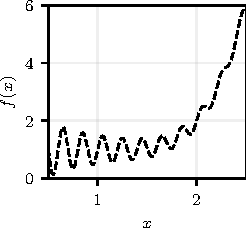
\includegraphics{../images/chap3_ex_gp_A.pdf} \hspace{3pt}
	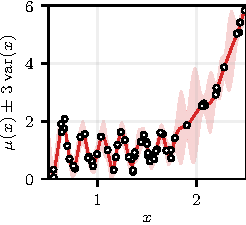
\includegraphics{../images/chap3_ex_gp_B.pdf} \hspace{3pt}
	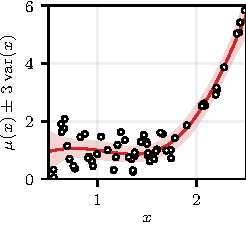
\includegraphics{../images/chap3_ex_gp_C.pdf} 
	\caption{A Gaussian process regression example. The ground-truth (left),  Gaussian process mean and the 3$\sigma$ confidence interval for a model with log marginal likelihood $\mathcal{L}=-29.8$ (middle) and $\mathcal{L}=-48.5$ (right).}
	\label{fig.chap3_gp_ex}
\end{figure}

An example of univariate Gaussian process regression is shown in Figure~\ref{fig.chap3_gp_ex}. The ground truth is a shifted Gramacy and Lee function $f(x) = \frac{\sin(10 \pi x)}{2x} + (x-1)^4 + 1$ from which 60 points were sampled with $\sigma \sim \mathcal{N}(0,0.15^2)$. The rational quadratic kernel was chosen to parametrize the GP covariance and the hyperparameters were tuned through MLE. The \texttt{GPflow} package \citep{matthews2017gpflow} was used in the numerical experiment and the objective was optimized through a BFGS method. In the figure, two distinct GP models are depicted, which were attained by means of MLE and BFGS under the same numerical tolerance and maximum number of iterations, but with different hyperparameter initial guesses. This illustrates how arriving at a favorable GPmodel through MLE requires escaping local maxima.

Up to this point, only ``static'' functions have been addressed and the GP modelling dynamical systems was not touched on. If the system under study is described by the familiar equations $x_{t+1} = f(x_t,u_t) + \epsilon$, $y_{t} = g(x_t) + \nu$ and the unknown $f$ is to be modelled from output data $y_t$ only, then the problem is difficult.  More precisely, even if $g$ is assumed linear and known, finding a closed-form posterior expression for $f$ is in general intractable and approximation schemes have to be used (e.g. variational inference or Markov-Chain Monte Carlo methods) \citep{turner2010state}. Tuning the hyperparameters in this so-called Gaussian process state-space model (GPSSM) setting is another non straightforward step \citep{eleftheriadis2017identification}. The control community has been working on making GPSSM computationally more efficient \citep{berntorp2021online} and even on understanding the properties of the learned dynamics \citep{beckers2016stability}, however an alternative approach exists that circumvents some of the aforementioned difficulties under an additional assumption. The method lies in modelling the unknown dynamics in an auto-regressive form and utilizing feature selection techniques and expert knowledge to decide on which signals and how many past samples to include, i.e., deciding what the regression vector should be. In such case, building a GP model for $x_{t+1} = f(x_t,u_t) + \epsilon$ reduces to learning a static map again as one would be assuming that full state measurement is possible. This was the direction taken in this investigation.

%In order to design dynamic models for the room temperatures, we used an auto-regressive approach, meaning that future predictions of a signal depend on the current and past values of itself as well as on current and past values of other relevant quantities. Since there were three temperatures to predict, three distinct models were trained and, so as to avoid augmenting the Gaussian process with unnecessary features, we made use of domain knowledge. Rooms that are not neighbors do not directly influence each other's temperatures; similarly, changing the valve position of AHU~1 has no effect on any temperature besides $T_1$. Initially, all exogenous signals $T_\text{sup}$, $T_\text{out}$ and $R_\text{sol}$ had been included into all models to boost their prediction capabilities. Nevertheless, we later realized that $R_\text{sol}$ was a significant covariate only for $T_3$ as discussed in Section~\ref{sec.ModelTrainingAndTesting}. Field tests unveiled a high correlation between the MPC computation times over the day and the solar radiation curve. Since having predictable rather than fluctuating solve times was a project requirement, we decided not to employ $R_\text{sol}$ as a feature in any GP. The definitive set of employed features is reported in Table~\ref{tab.features}, where the delay parameter $l$ indicates the number of current plus past values used from that particular physical signal. By using the mean functions \eqref{eq.GPmean} to evolve the temperature dynamics, we arrive at the final models
%\begin{subequations}
%	\begin{align}
%		T_{1,t+1} &= \mu_{1}(T_{1,t}, T_{1,t-1}, T_{2,t}, \theta_{1,t},T_{\text{sup},t},T_{\text{out},t}) \\
%		T_{2,t+1} &= \mu_{2}(T_{1,t}, T_{2,t}, T_{2,t-1}, T_{3,t}, \theta_{2,t},T_{\text{sup},t},T_{\text{out},t}) \\
%		T_{3,t+1} &= \mu_{3}(T_{2,t}, T_{3,t}, T_{3,t-1}, \theta_{3,t},T_{\text{sup},t},T_{\text{out},t}) 
%	\end{align}
%	\label{eq.GPmodels}
%\end{subequations}
%Concerning the variances \eqref{eq.GPvar}, we opted for not propagating them forward in time since no closed-form expression exists to accomplish this. Instead, the expression \eqref{eq.GPvar} was evaluated in a point-wise fashion to measure uncertainty. The interested reader is referred to \cite{girard2004approximate,mchutchon2011gaussian} for insightful discussions on the matter.

\section{The building and its HVAC system}
\label{sec.building_and_hvac}

The building considered in this study was a surgery center situated in the São Julião hospital complex, in the city of Campo Grande, MS, Brazil (Figure~\ref{fig.facadeAndRooms}, top). The 51 rooms that compose it are in permanent use and, for information purposes, 528 surgical procedures were carried out in it during August 2021. We were concerned with three thermal zones in its ophthalmology section: two operating rooms (ORs) and one waiting room (WR), all located on the West end of the building (Figure~\ref{fig.facadeAndRooms}, bottom). Whereas the former rooms are only connected to the waiting room, the latter has a door to the rest of the surgery center. Opaque glass bricks are present in the waiting room as can be seen in the picture, allowing some natural light to enter the space; the operating rooms on the other hand do not feature them, nor do they have any windows. All spaces have exterior walls, but the right-hand side operating room is significantly more affected by direct solar radiation due to the disposition of the nearby trees.

\begin{figure}[!t]
	\centering
	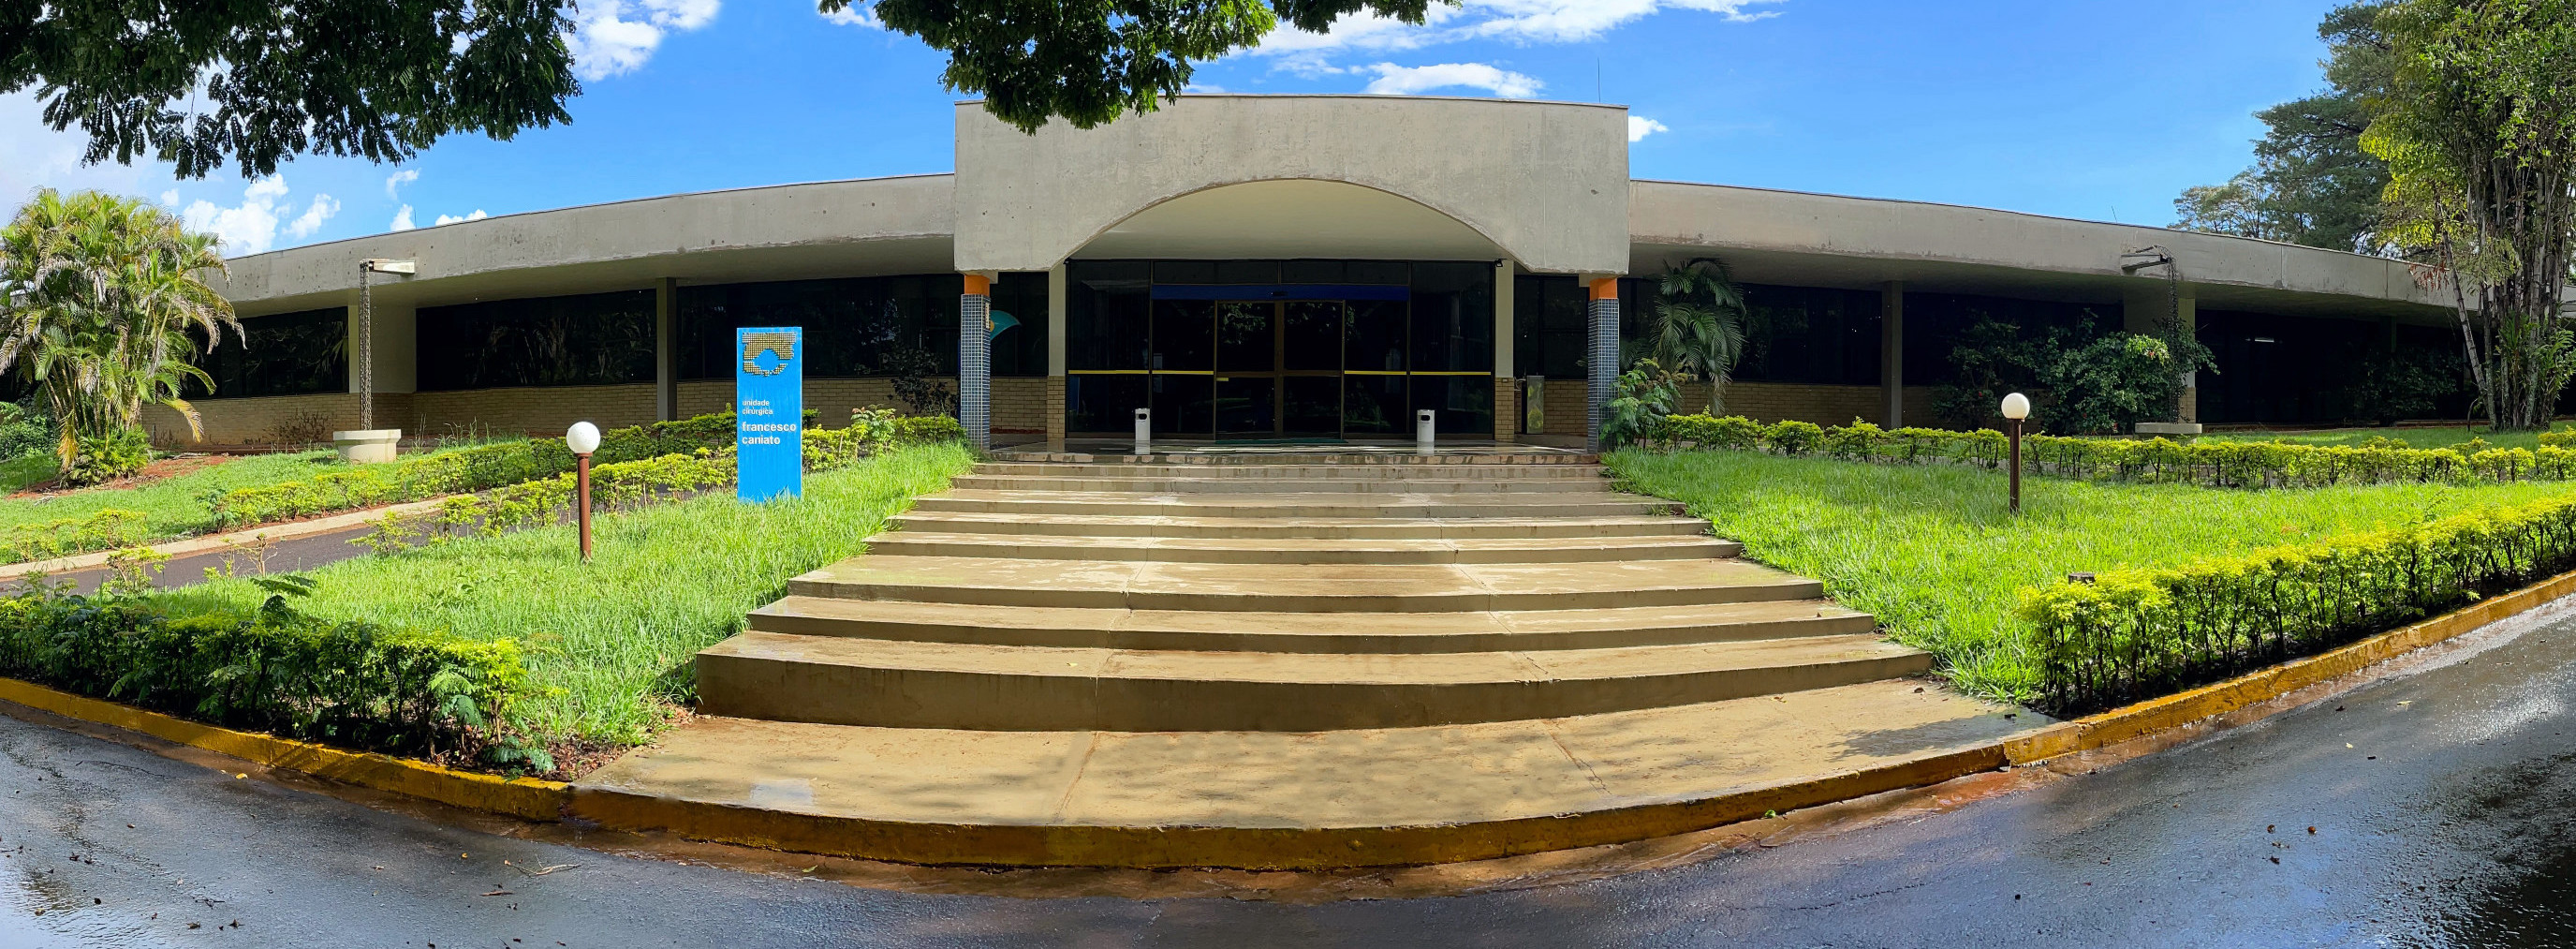
\includegraphics[width=0.9\linewidth]{../images/chap3_facade.jpg} \\[8pt]
	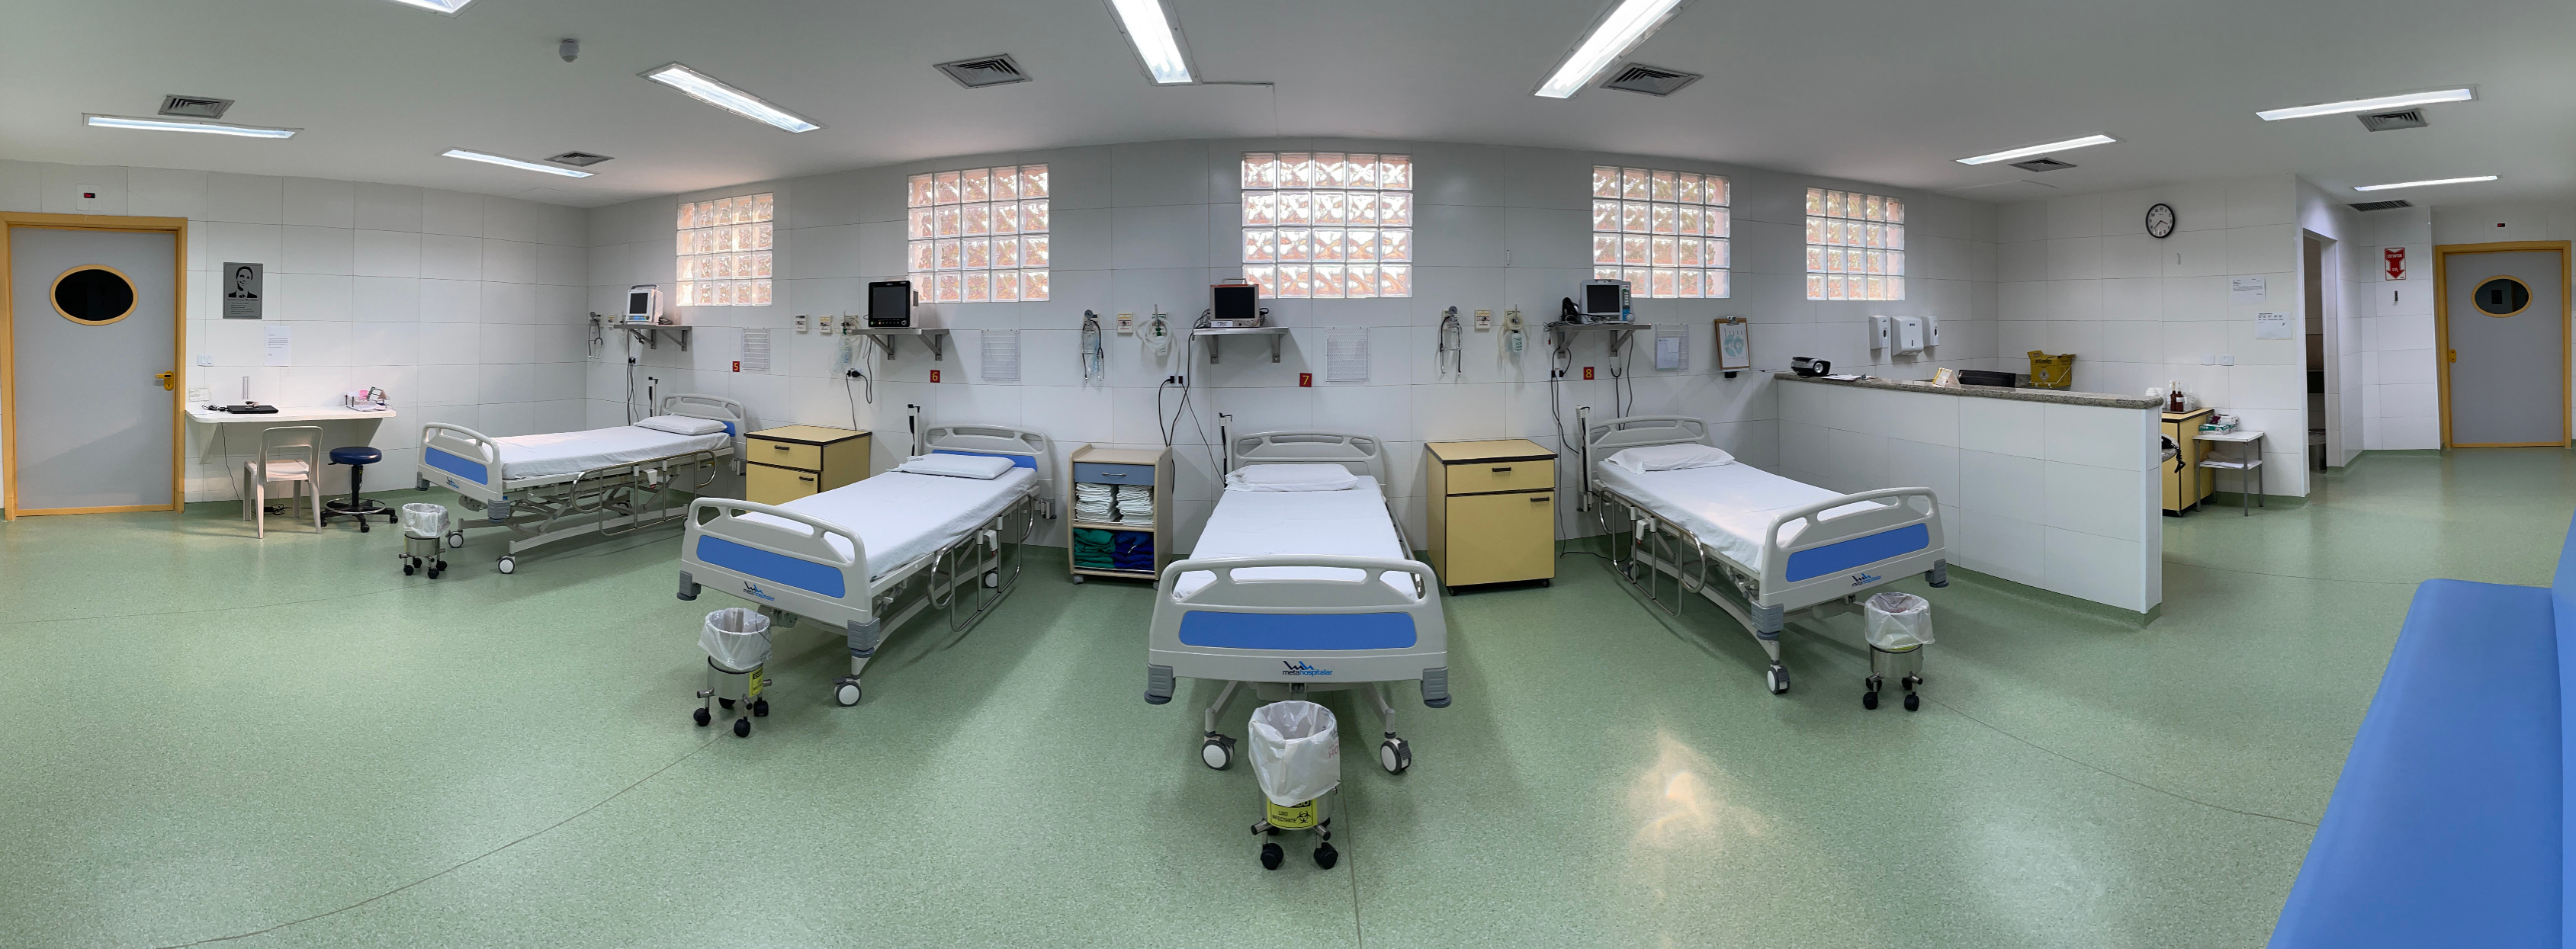
\includegraphics[width=0.9\linewidth]{../images/chap3_rooms.jpg} 
	\caption{The facade of the Hospital São Julião surgery center, situated in Campo Grande, MS, Brazil (top). The three thermal zones considered in this study (bottom): The waiting room and the doors that lead to the two operating rooms, all in the ophthalmology section of the building, located on its West end.}
	\label{fig.facadeAndRooms}
\end{figure}

A forced-air cooling plant is in place to provide the occupants with a suitable indoor climate in accordance with local regulations. A total of seven \acp{ahu} collect outdoor air that is then treated and filtered before being pumped into the several indoor spaces. We had control only over three \acp{ahu}, one for each aforementioned thermal zone. A central chiller connected to an external cooling tower provides chilled water to all \acp{ahu}, which in turn feature three-way valves to control the flow of water through their cooling coils. The \ac{ahu} fans are operated always at constant speed, resulting in a constant volumetric flow through the air-ducts and into the zones. As per the regulations, no air recycling is possible and all return air is directly discharged into the atmosphere. As the temperature in Campo Grande is typically high, the \ac{hvac} system was conceived to only cool the space, not having the means to provide positive thermal energy (for more details, see Section~\ref{sec.controlProb}).

\begin{figure}[!t]
	\centering
	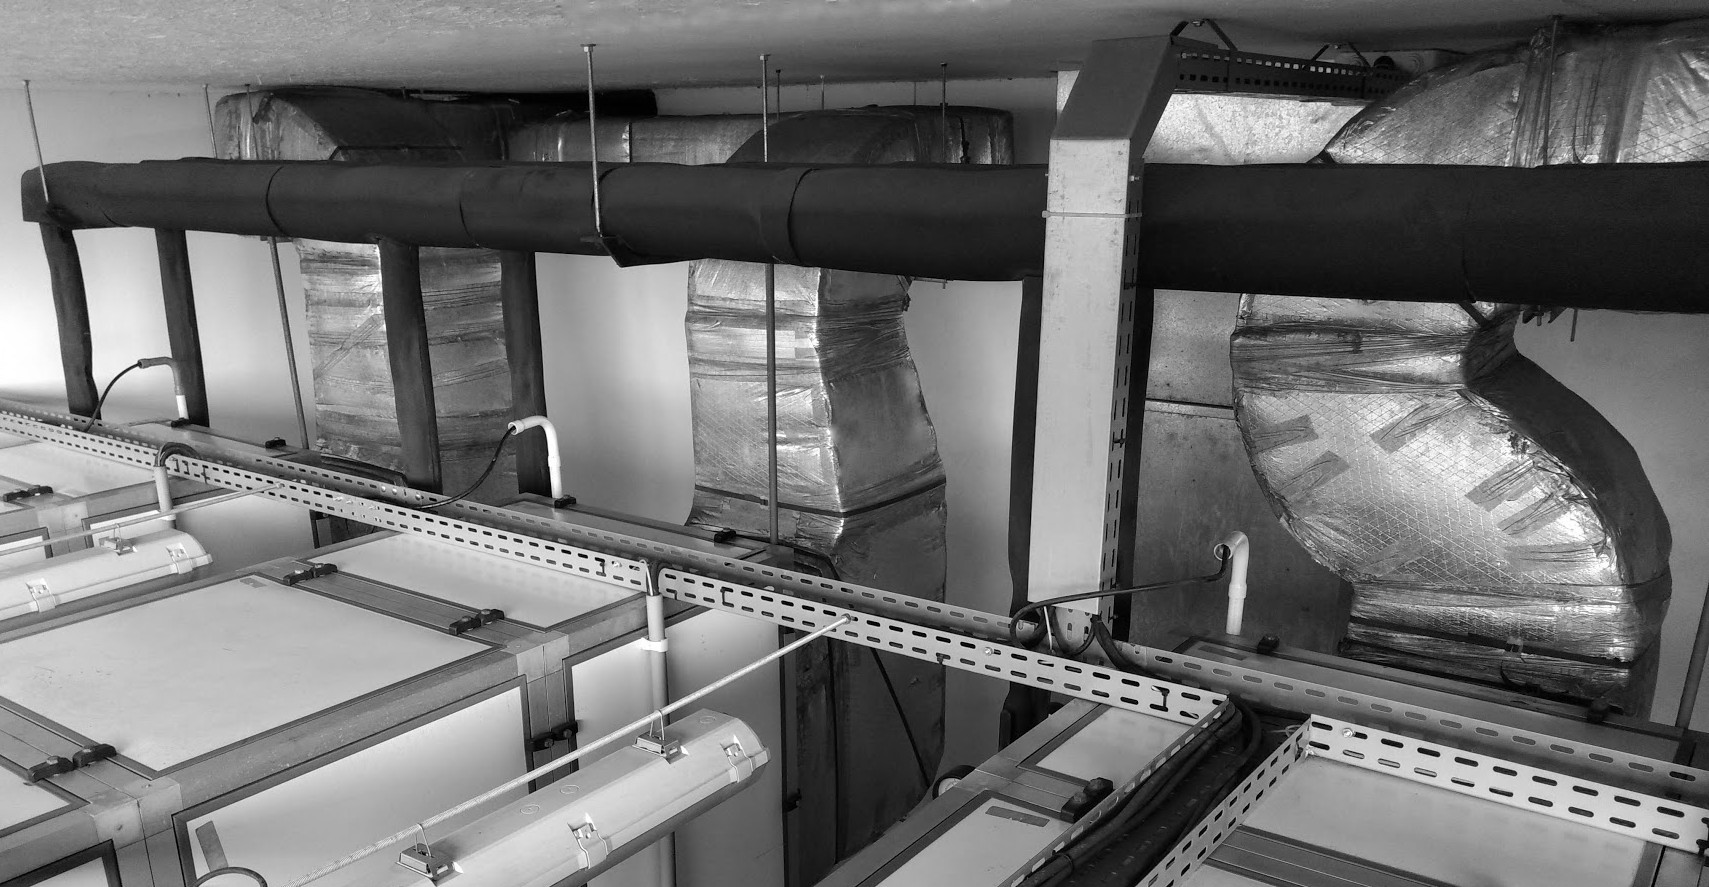
\includegraphics[width=0.75\linewidth]{../images/chap3_ahus_b.jpg} \\[8pt]
	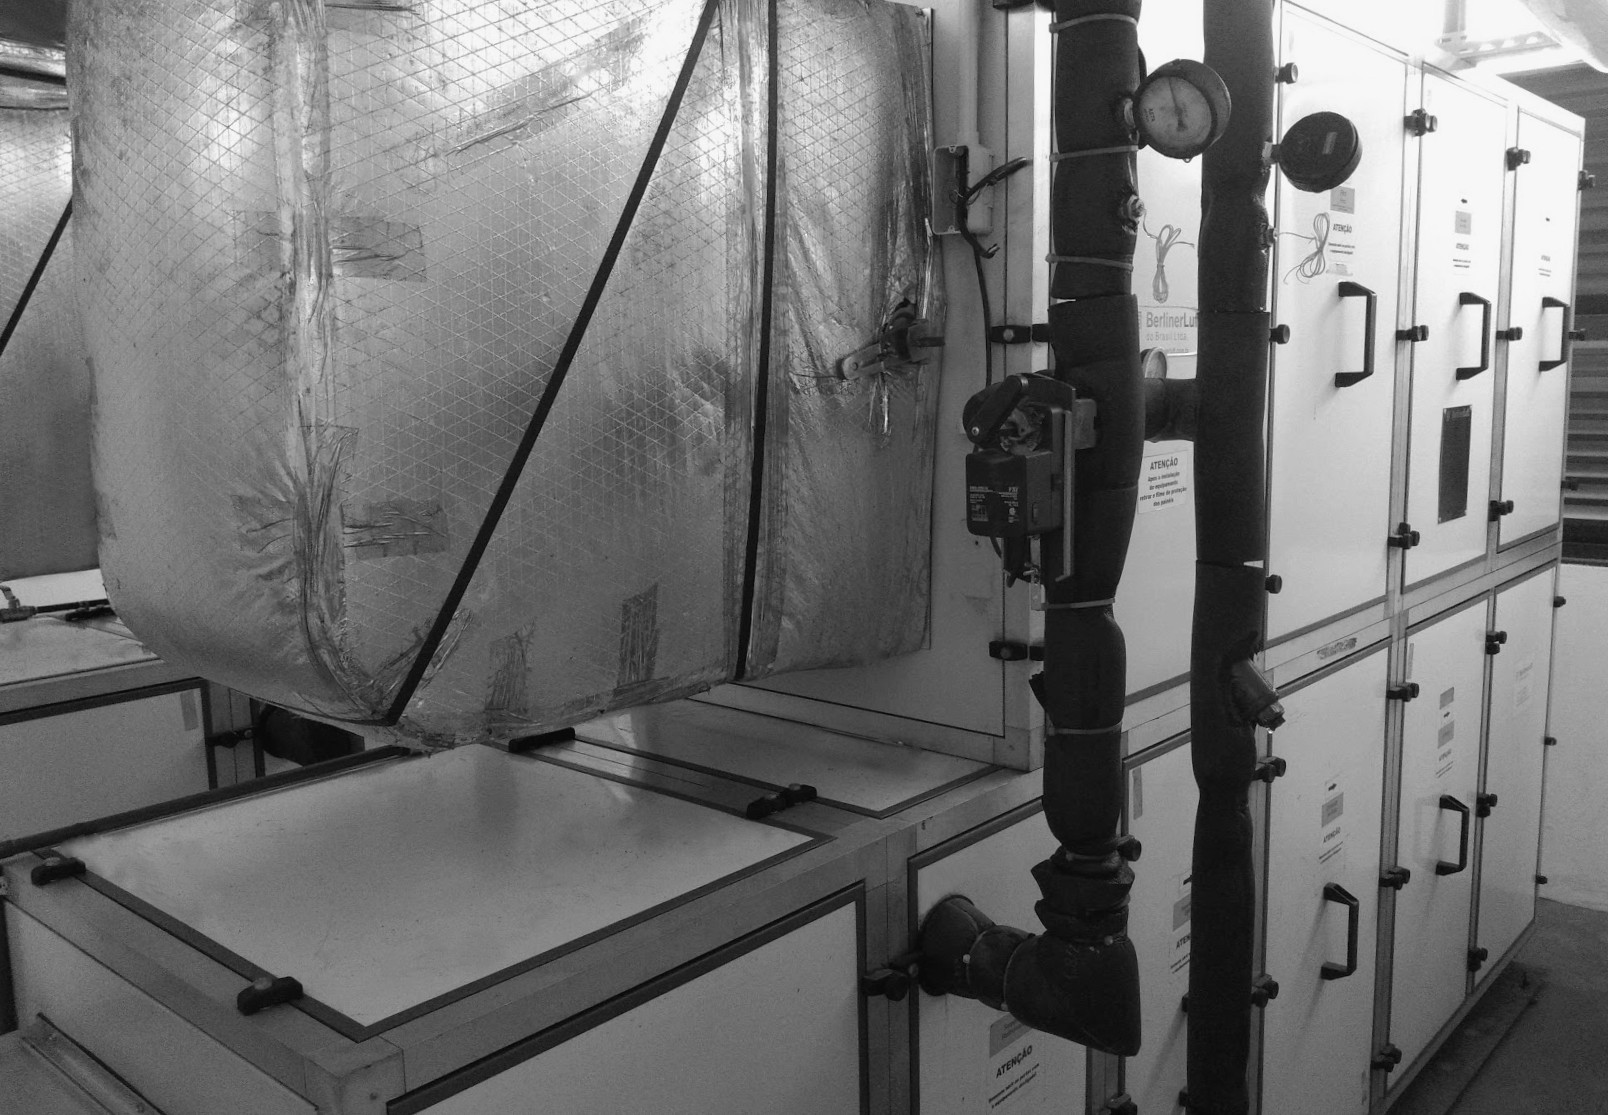
\includegraphics[width=0.75\linewidth]{../images/chap3_ahus_a.jpg} 
	\caption{Photos of the \ac{ahu} room where one can identify the air ducts (top), the supply and return water pipes (top and bottom), and one of the three-way valve servomotors that control the flow of chilled water (bottom).}
	\label{fig.ahuRoom}
\end{figure}

Two distinct sensor networks were deployed to monitor the \ac{hvac} plant and the indoor spaces. Firstly, we will describe the one located in the \ac{ahu} room. One local controller (LCO)--a National Instruments myRIO--was attached to each air-handling unit to read all sensors and monitor the \acp{ahu}: supply and return water temperature probes, a water flow meter, an anemometer, as well as an angular position sensor. The LCOs were moreover responsible for running low-level signal processing routines and implementing control actions, i.e., acting on the three-way valve servomotor to change the chilled water flow, hence influencing the supply air temperature. Photos of the \ac{ahu} room are shown in Figure~\ref{fig.ahuRoom}. Next, in order to measure the indoor temperatures in a flexible way, a wireless network of Z-wave sensors was set up in the operating rooms and waiting room. These were equipped with external temperature probes (Dallas DS18B20) to guarantee fast and precise readings, reporting their measurements periodically to a local computer (LC) that featured a Z-wave transceiver attached to it.

%They periodically report they samples to a 2.66~GHz Mac Mini equipped with a Z-wave USB transceiver that was installed in the waiting room. This local computer (LC) acted as the main computing platform for the project, gathering data from all sources, hosting a local database, and running all the real-time optimization algorithms.
The LC was a 3~GHz, 16 GB RAM, core i7 machine installed in the waiting room and acting as the main computer platform for the project. This computer and the \ac{ahu} LCOs were all connected to a local area network (LAN) to exchange information, which was done by using the UDP protocol at a rate of 1~Hz. We highlight that this same LAN was used to send control signals from the LC to the LCOs in order to modulate the \ac{ahu} valves. Lastly, a weather station was deployed on site to measure the outdoor temperature and the solar radiation acting on the building with high accuracy. All signals were sampled with a period of two minutes and stored into a local time-series database, InfluxDB. A block-diagram of the complete system is depicted in Figure~\ref{fig.blockDiagram}.  

\begin{figure}[!t]
	\centering
	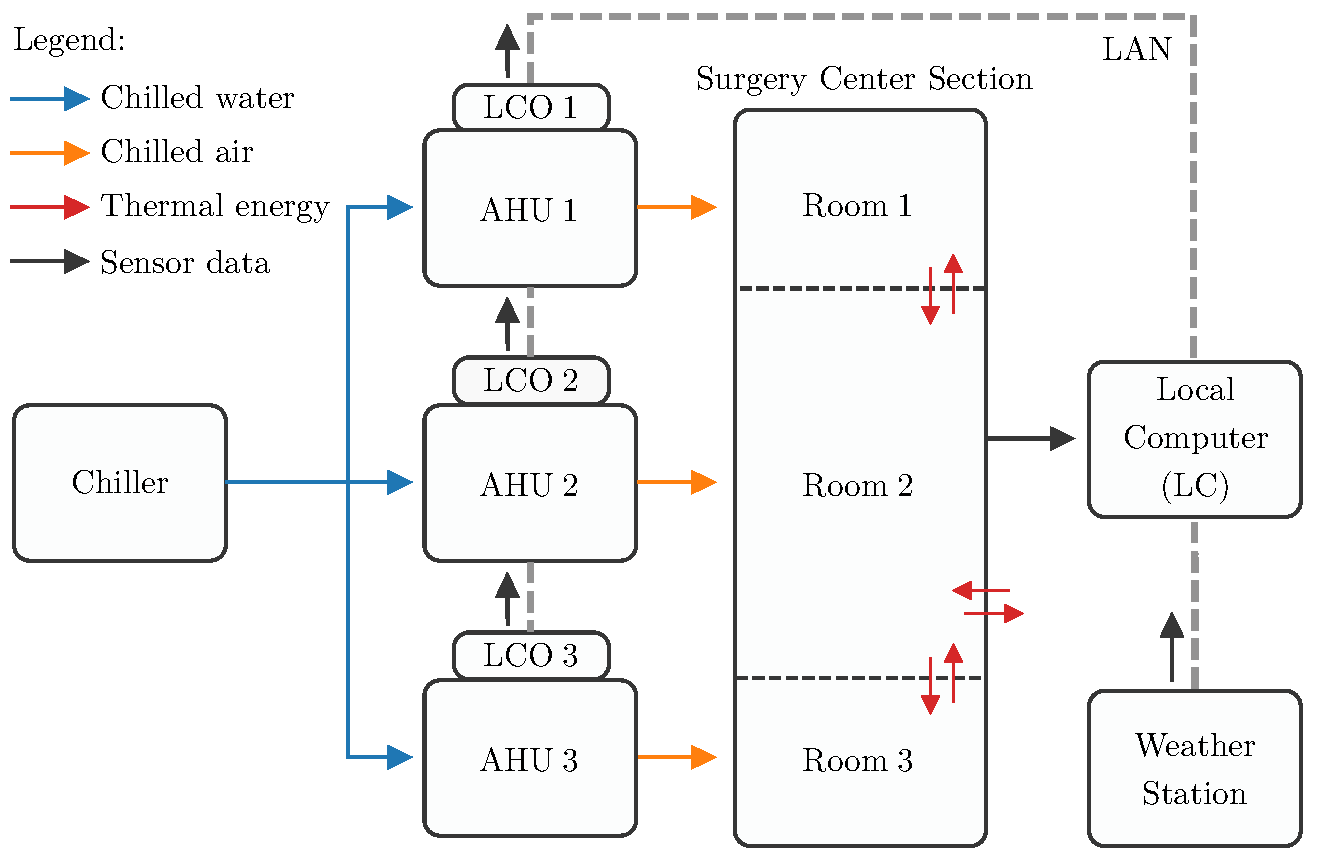
\includegraphics[width=0.75\linewidth]{../images/chap3_sys_arch_diagram.pdf}
	\caption{The overall system architecture, including the three \acp{ahu} and their local controllers (LCOs). Information is exchanged between the LCOs and the local computer (LC) through a local area network (LAN).}
	\label{fig.blockDiagram}
\end{figure}

\subsection{Analysis of the control problem}
\label{sec.controlProb}

The control goal was to regulate the indoor temperature within the three zones ($T_i$, $i=1,2,3$), keeping it below a pre-specified value $T_{\text{max}}$ at all times. Although defining two-level temperature envelopes that have relaxed constraints at night is common for residences and offices, some employees still made use of the surgery center spaces during nighttime and, thus, the indoor temperature has to stay below $T_{\text{max}}$ even then. Furthermore, this was to be done while minimizing the chiller energy consumption, which is a function of its coefficient of performance (COP) curve and the building thermal load. 

The controlled variables are the angular positions of each \ac{ahu} three-way valve ($\theta_i$, $i=1,2,3$) that regulate the flow of water across their cooling coils. Naturally, these quantities are physically limited between a minimum $\theta_\text{min}$ and a maximum value $\theta_\text{max}$. Several disturbances both of internal and external nature act on the system. The measured ones include the outdoor temperature $T_\text{out}$, the solar radiation $R_\text{sol}$, and the temperature of the water supplied by the chiller to the \acp{ahu}, $T_\text{sup}$. The variables $T_\text{out}$ and $R_\text{sol}$ directly affect the indoor climate by heating the external walls. Also, both $T_\text{out}$ and $T_\text{sup}$ can be regarded as input disturbances; indeed, these quantities define the \ac{hvac} system actuation capabilities along with the valve positions $\theta_i$. The unmeasured disturbances are the internal heat gains generated by occupants and equipment, as well as the eventual opening and closing of doors that lead to air mix among rooms. A summary of the relevant control information described here can be found in Table~\ref{tab.controlInformation}.


In order to operate optimally the industrial cooling system while minimizing the operational costs, we opted for designing and recursively solving a model-based finite-horizon optimal control problem. To craft dynamical models for the temperature evolution in the rooms and the \ac{ahu} effects on them, we made use of the Gaussian process framework described in Section~\ref{sec.gps}.
%ional to the angular position. For this reason, we decided to adopt a flexible class of statistical models to tackle the modeling problem while requiring as little expert knowledge as possible. Their main advantage being that this class not only predicts the expected system behavior, but also quantifies the uncertainty associated with its predictions, hence allowing for a more robust, risk-aware operation.

\subsection{Data collection, model training and testing}
\label{sec.ModelTrainingAndTesting}

Aiming at capturing different weather conditions and a reasonable number of chiller states, a representative dataset was gathered from August to November 2021. The batch consisted of 22'455 points sampled at $T_\text{samp} = 2\,$ mins and comprised closed-loop operation with PI and rule-based controllers (RBCs), as well as a variety of open-loop excitation signals such as ramps and uniformly random inputs. The latter signals were mainly tested during weekends and Holidays to avoid disturbing occupants. After examining the obtained curves, we concluded that a control period of 10 mins would be a good compromise between operating the cooling system effectively and not oversampling the temperatures -- given that our model complexity grows with the size of the dataset, the latter aspect was rather important. The dataset was then downsampled by a factor of 5 times, resulting in 4'491 points, which corresponds to 748 hours. 

A meticulous post-processing step was necessary next to ensure that unreliable periods were discarded. We highlight that this was not simply a matter of finding spurious outliers, but of identifying complete periods of time when the plant was not operating normally due to, for instance, a chiller fault, an unannounced maintenance in an \ac{ahu} or even the manual closing of some air dampers by a technician. This process was carried out by jointly studying the obtained curves with the help of the local maintenance team. Finally, missing entries in the time-series were imputed using a simple linear interpolation scheme. Thanks to the reliability of the sensor networks shown in Section~\ref{sec.building_and_hvac}, only a small percentage of entries was not present. With the right set of data at hand, we proceeded to define and train one GP model for each room. 

\begin{table}
	\small
	\centering
	\caption{The main physical quantities influencing the \ac{hvac} plant and the temperature dynamics inside the rooms.}
	\label{tab.controlInformation}
	\begin{tabular}{l c c} 
		\cmidrule[.15em](l{\tabcolsep}r{\tabcolsep}){1-3}
		& Symbols & Description \\
		\cmidrule[.15em](l{\tabcolsep}r{\tabcolsep}){1-3}
		Inputs & $\theta_\text{1}$, $\theta_\text{2}$, $\theta_\text{3}$ & \makecell{Valve position of \ac{ahu} 1, \\ \ac{ahu} 2 and \ac{ahu} 3} \\
		\cmidrule[.05em](l{\tabcolsep}r{\tabcolsep}){1-3}
		Outputs & $T_\text{1}$, $T_\text{2}$, $T_\text{3}$ & \makecell{Temperatures within zone 1,  \\ zone 2 and zone 3} \\
		\cmidrule[.05em](l{\tabcolsep}r{\tabcolsep}){1-3}
		Measured disturbance & $T_\text{sup}$, $T_\text{out}$, $R_\text{sol}$ & \makecell{Chiller supply water temperature, \\ outdoor temperature, solar radiation} \\
		\cmidrule[.05em](l{\tabcolsep}r{\tabcolsep}){1-3}
		Unmeasured disturbance & $-$ & \makecell{Internal heat gains (e.g. occupants), \\ opening and closing of doors} \\
		\cmidrule[.15em](l{\tabcolsep}r{\tabcolsep}){1-3}
	\end{tabular}
\end{table}

\begin{table}[!t]
	\small
	\centering
	\caption{Delays for each feature of the Gaussian process auto-regressive models. The symbol ``$-$'' indicates what signals were neglected.}
	\begin{tabular}{l c c c c c c c c}
		\cmidrule[.15em](l{\tabcolsep}r{\tabcolsep}){1-9}
		& $T_\text{1}$ & $T_\text{2}$ & $T_\text{3}$ & $\theta_\text{1}$ & $\theta_\text{2}$ & $\theta_\text{3}$ & $T_\text{sup}$ & $T_\text{out}$ \\
		\cmidrule[.15em](l{\tabcolsep}r{\tabcolsep}){1-9}
		GP1 (OR 1) & 2 & 1 & $-$ & 1 & $-$ & $-$ & 1 & 1 \\
		\cmidrule[.05em](l{\tabcolsep}r{\tabcolsep}){1-9}
		GP2 (WR) & 1 & 2 & 1 & $-$ & 1 & $-$ & 1 & 1 \\
		\cmidrule[.05em](l{\tabcolsep}r{\tabcolsep}){1-9}
		GP3 (OR 2) & $-$ & 1 & 2 & $-$ & $-$ & 1 & 1 & 1 \\
		\cmidrule[.15em](l{\tabcolsep}r{\tabcolsep}){1-9}
	\end{tabular}
	\label{tab.features}
\end{table}

The process of designing GP models can be summarized in three steps: select suitable mean and covariance functions, define the feature vectors, and optimize the models hyperparameters. Among the many kernel maps available in the literature, we chose the anisotropic squared-exponential function, a very popular alternative due to its smoothness and expressive power. This kernel has the form
\begin{equation}
	k_{\text{SE}}(x,x') = \sigma^2 \exp \left(-\frac{1}{2} \sum_{i=1}^d \left(\frac{x_i - x'_i}{\ell_i}\right)^2\right)
	\label{eq.SEARD}
\end{equation}
where $x_i$ is the $i$th component of the feature vector $x$. In \eqref{eq.SEARD}, $\sigma$ is the so called vertical scale hyperparameter and $\ell_i$ are the horizontal scale (a.k.a. lengthscale) hyperparameters. However, relying solely on \eqref{eq.SEARD} can be dangerous as the resulting GP model would not extrapolate well. For this reason, a linear mean function $m(x) = Ax + b$ was also employed, causing the Gaussian process to behave linearly when far away from the training data. As for optimizing the hyperparameters we made use of the log-marginal likelihood objective and the Broyden–Fletcher–Goldfarb–Shanno (BFGS) first-order algorithm. The development was carried out in \texttt{Python} with the aid of the \texttt{GPflow2} \citep{matthews2017gpflow} and the \texttt{SciPy} \citep{virtanen2020scipy} packages.

To model the temperature dynamics in the rooms, an auto-regressive structure was preferred over a state-space one (see discussion in Section~\ref{sec.gps}). In other words, future predictions of a signal depend on the current and past values of itself as well as on current and past values of other relevant quantities. Since there were three temperatures to predict, three distinct GPs were trained and, to avoid augmenting the Gaussian process with unnecessary features, we made use of domain knowledge. Rooms that are not neighbors do not directly influence each other's temperatures; similarly, changing the valve position of \ac{ahu}~1 has no effect on any temperature besides $T_1$. Initially, all exogenous signals $T_\text{sup}$, $T_\text{out}$ and $R_\text{sol}$ had been included into all models to boost their prediction capabilities. Nevertheless, we later realized that $R_\text{sol}$ was a significant covariate only for $T_3$. Field tests also unveiled a high correlation between the MPC computation times over the day and the solar radiation curve. Since having consistent rather than fluctuating solve times was a project requirement, we decided not to employ $R_\text{sol}$ as a feature in any GP. The definitive set of features and signal delays is reported in Table~\ref{tab.features}. Finally, by using the mean functions \eqref{eq.GPmodels} to evolve the temperature dynamics, we arrive at the final models
\begin{subequations}
	\begin{align}
		T_{1,t+1} &= \mu_{1}(T_{1,t}, T_{1,t-1}, T_{2,t}, \theta_{1,t},T_{\text{sup},t},T_{\text{out},t}) \\
		T_{2,t+1} &= \mu_{2}(T_{1,t}, T_{2,t}, T_{2,t-1}, T_{3,t}, \theta_{2,t},T_{\text{sup},t},T_{\text{out},t}) \\
		T_{3,t+1} &= \mu_{3}(T_{2,t}, T_{3,t}, T_{3,t-1}, \theta_{3,t},T_{\text{sup},t},T_{\text{out},t}) 
	\end{align}
	\label{eq.GPmodels}
\end{subequations}
Regarding the variances \eqref{eq.gp_variance}, those were used in a point-wise fashion to measure uncertainty. In other words, multi-step ahead predictions were performed by propagating only the mean values forward. The more complex alternative, which was discarded in this study, is to propagate also the higher-order moments and employ numerical methods to approximate the intractable integrals in the hope of arriving at more precise uncertainty estimates \citep{girard2004approximate,mchutchon2011gaussian}.

\afterpage{
\begin{landscape}
\begin{figure*}[!t]
	\centering
	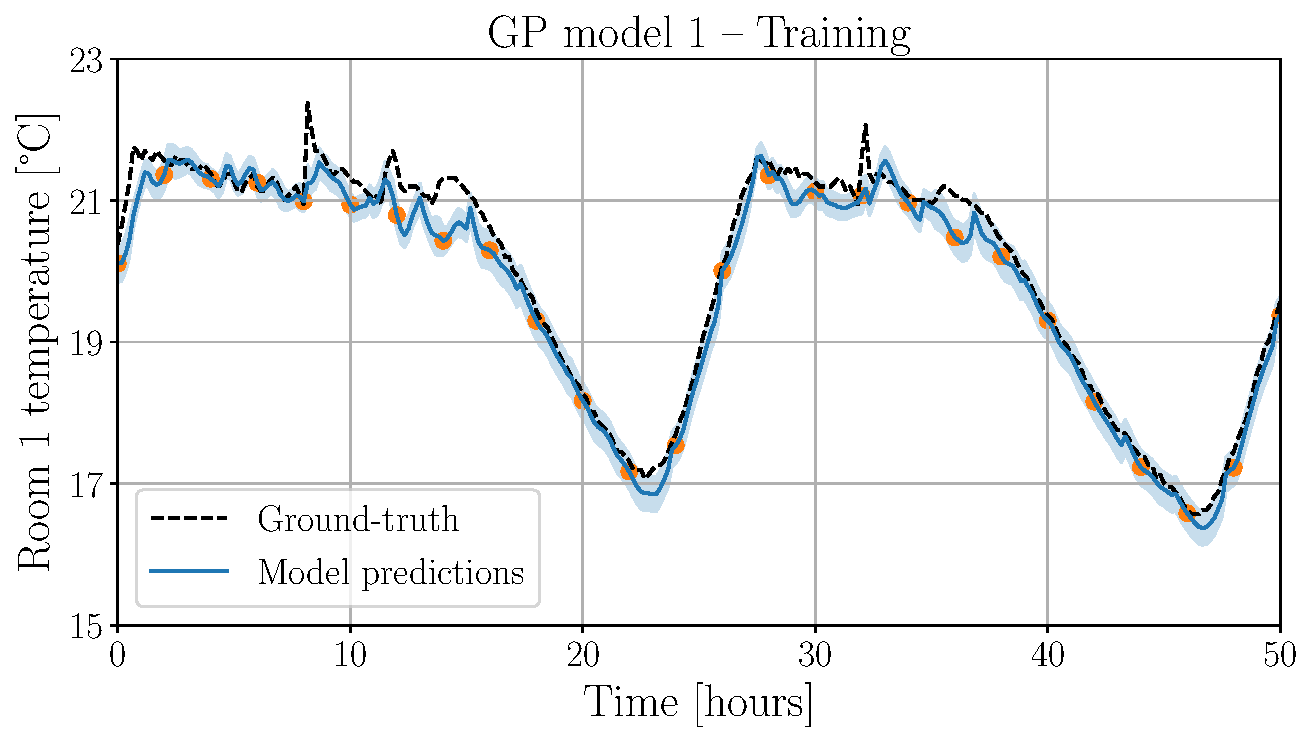
\includegraphics[scale=0.29]{../images/chap3_room_1_temp_model_train.pdf}  
	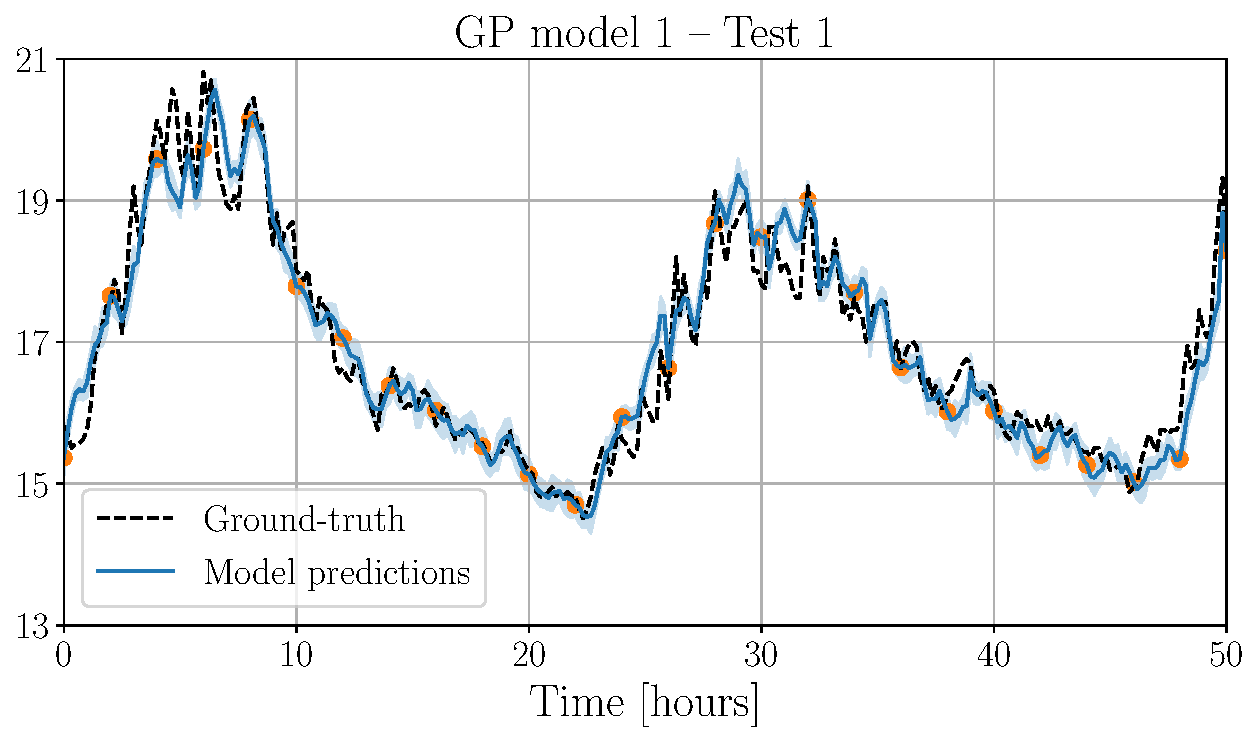
\includegraphics[scale=0.29]{../images/chap3_room_1_temp_model_test1.pdf} 
	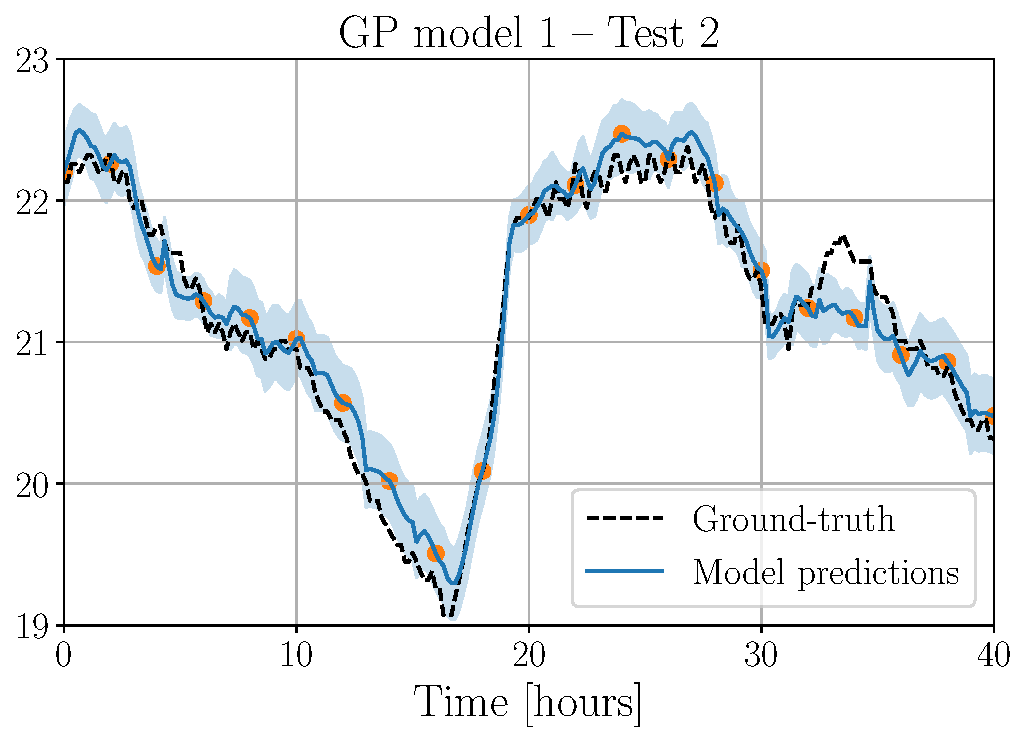
\includegraphics[scale=0.29]{../images/chap3_room_1_temp_model_test2.pdf} \\[10pt]
	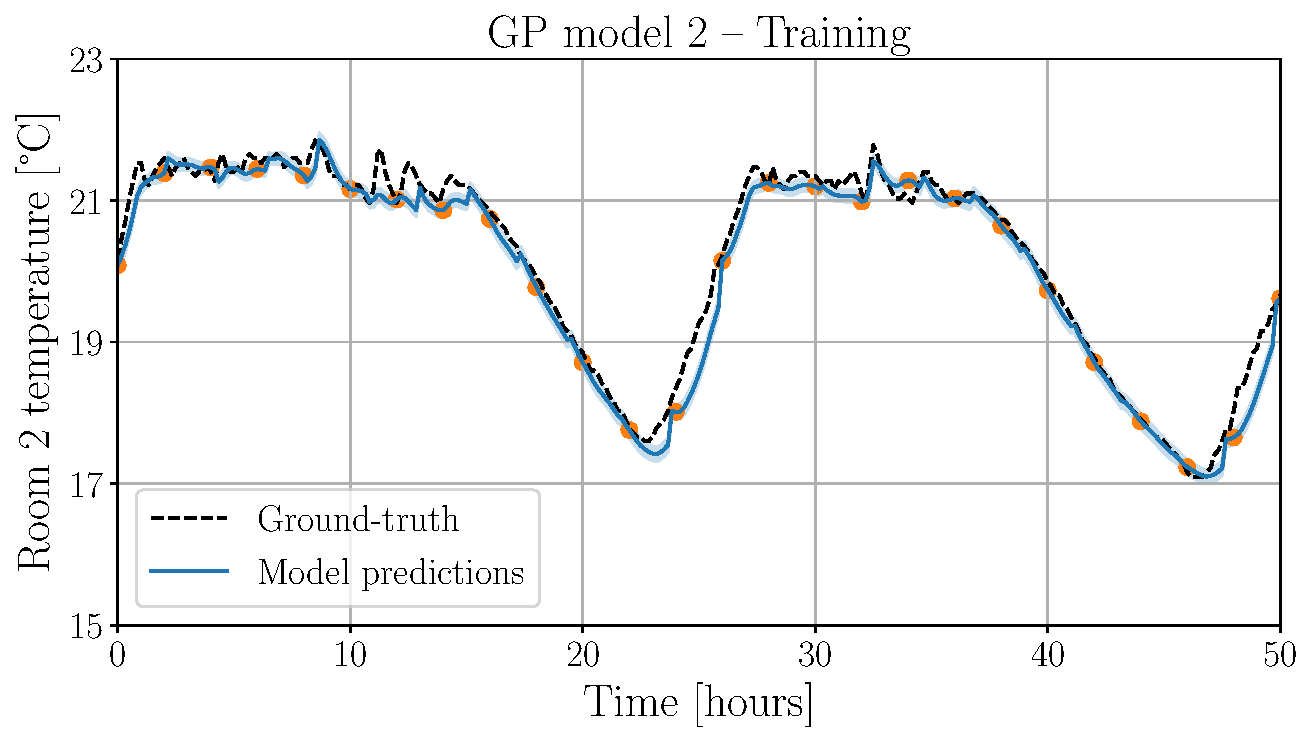
\includegraphics[scale=0.29]{../images/chap3_room_2_temp_model_train.pdf} 
	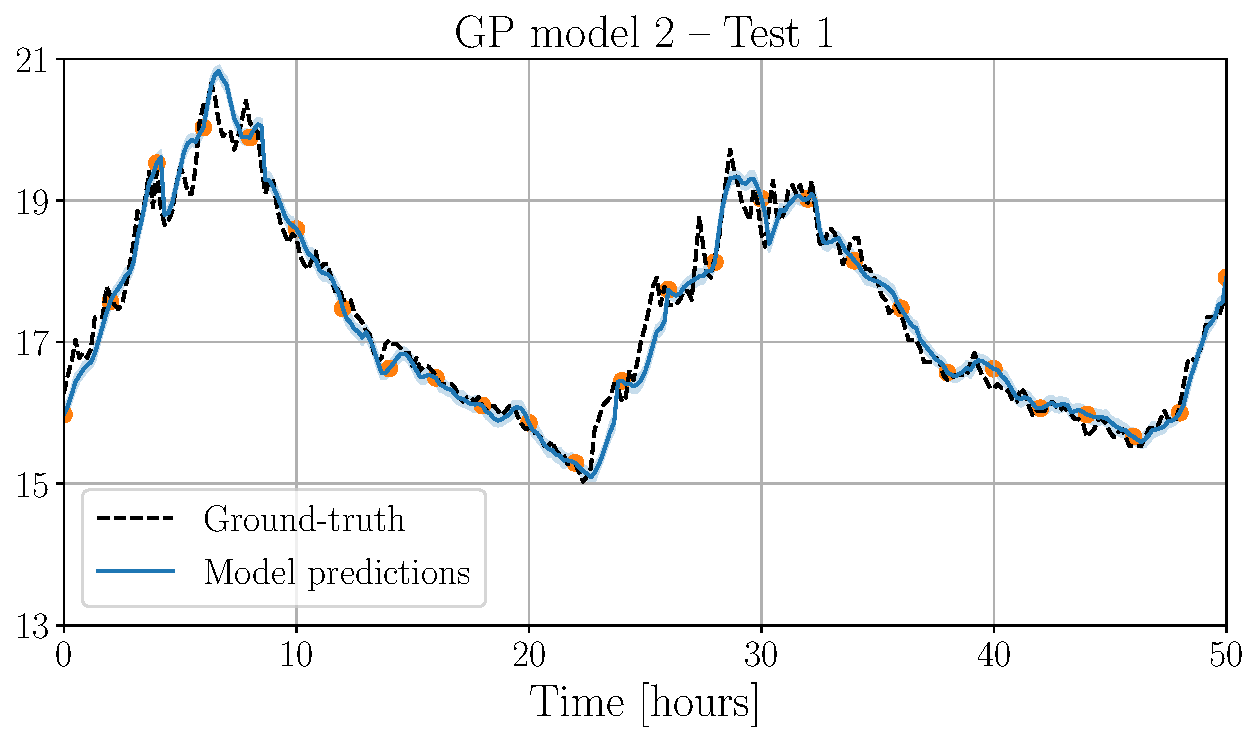
\includegraphics[scale=0.29]{../images/chap3_room_2_temp_model_test1.pdf}
	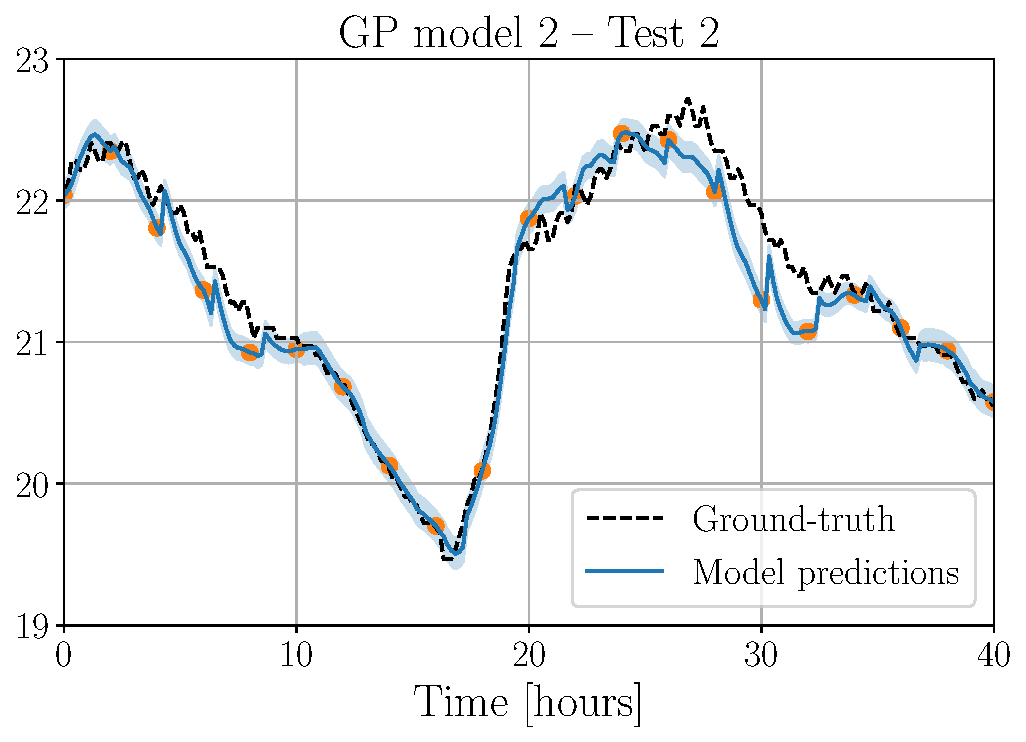
\includegraphics[scale=0.29]{../images/chap3_room_2_temp_model_test2.pdf} \\[10pt]
	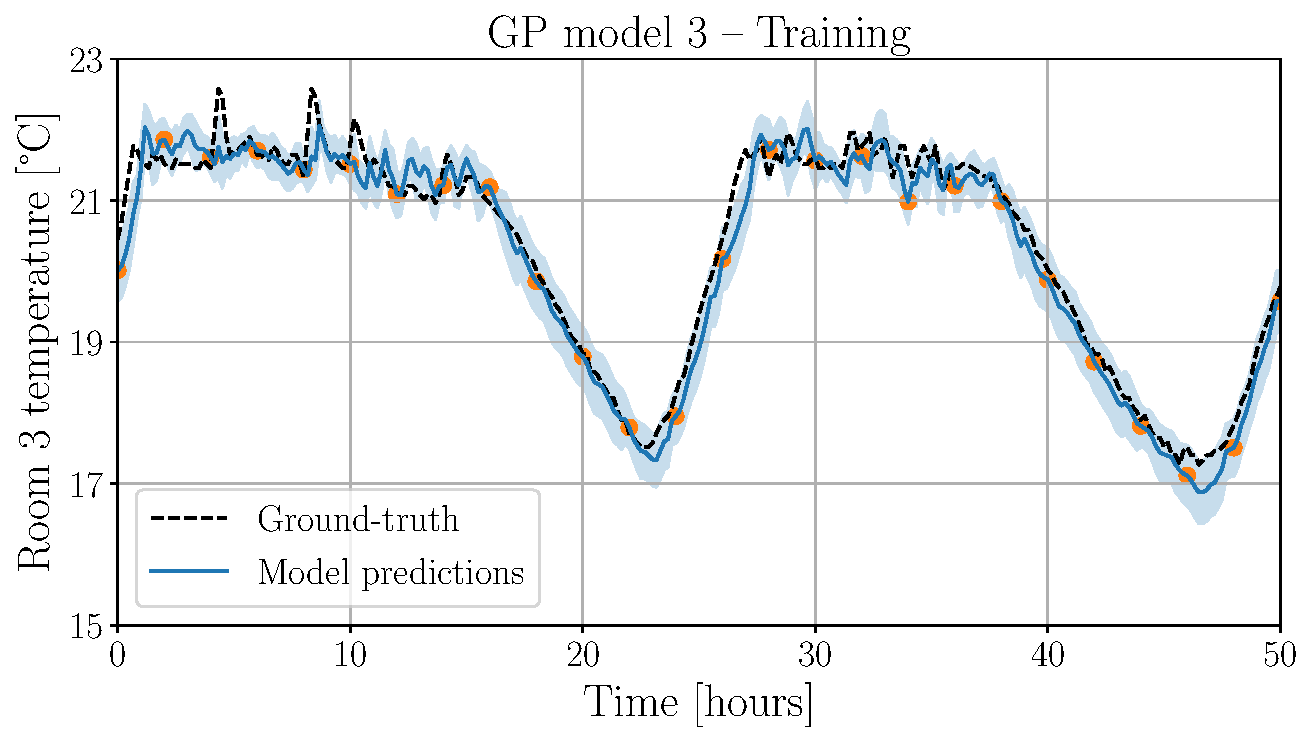
\includegraphics[scale=0.29]{../images/chap3_room_3_temp_model_train.pdf} 
	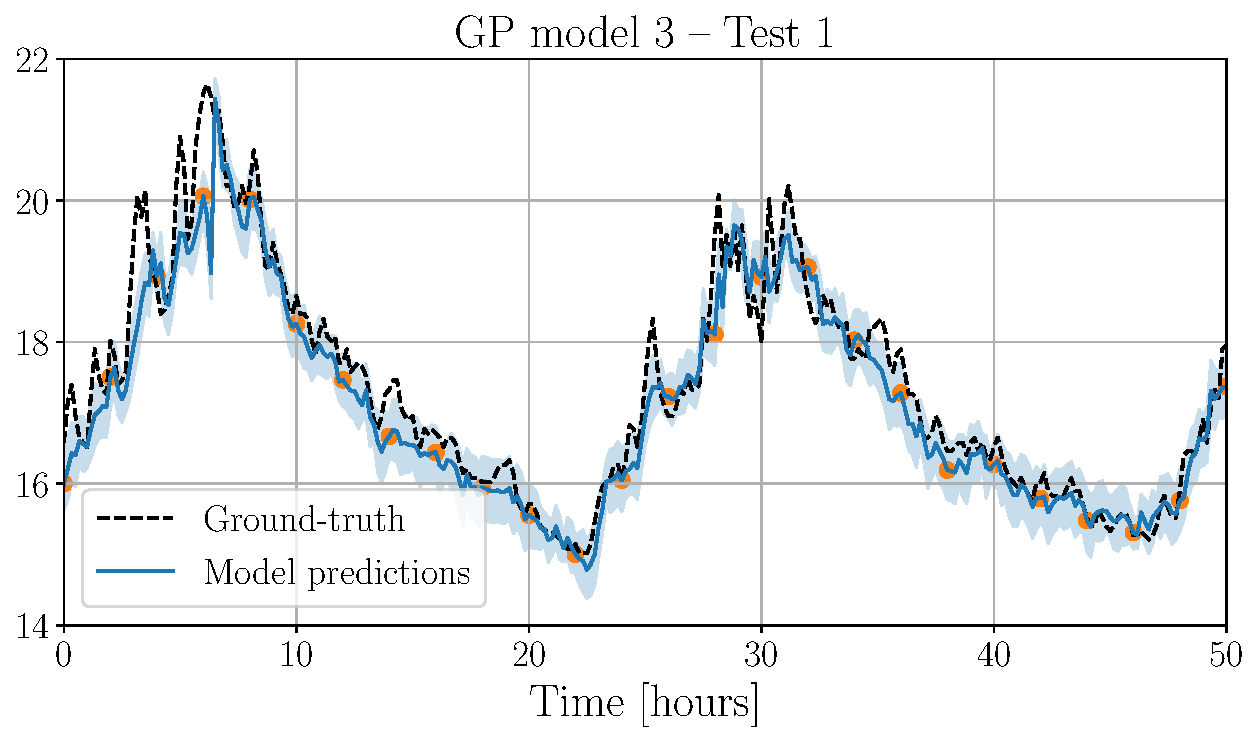
\includegraphics[scale=0.29]{../images/chap3_room_3_temp_model_test1.pdf}
	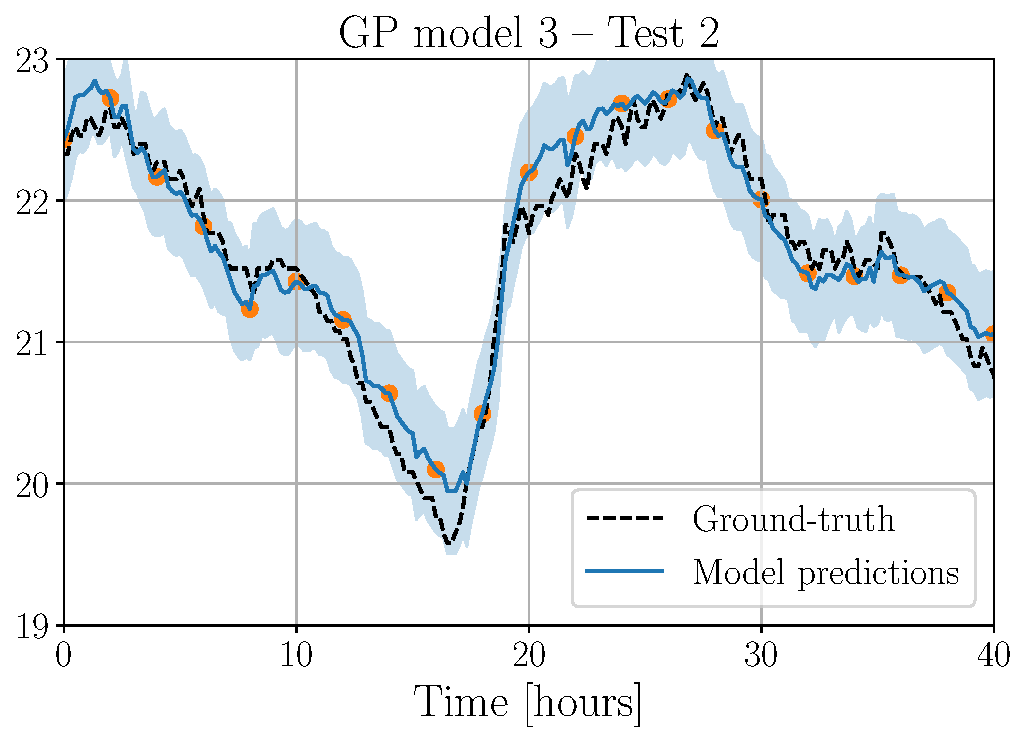
\includegraphics[scale=0.29]{../images/chap3_room_3_temp_model_test2.pdf}
	\caption{
		Train and test results for the Gaussian process auto-regressive models predicting the temperature evolution within rooms 1, 2 and 3. The training plots only display a portion of the training set. The GP means are depicted in solid blue and the two standard deviation interval in light blue. The real temperatures are shown in dashed black.
		%Training (left) and test results (center, right) of the Gaussian process models based on real experimental data. The mean predictions are shown in solid blue, whereas the uncertainty envelope of two standard deviations, in light blue. The sampling period is 10 minutes. The mean predictions were obtained by simulating the GP auto-regressive models forward in time for 2 hours and only feeding back new temperature information at the orange dots. The training plots only show a portion of the training set.
	}
	\label{fig.trainTestRes}
\end{figure*}
\end{landscape}
}

In order to train the GP models in an efficient way, balancing the information brought by the data-set and non-parametric model size, nearby feature vectors were dropped. The Euclidean norm of the difference was chosen as the distance function. Such a dropping also improves the numerical stability of the model kernel matrix. Finally, the GPs modeling rooms 1, 2 and 3 had respectively 235, 245 and 314 points, which correspond to approximately 38, 51 and 47 hours worth of data. Since these sets did not come from a single experiment, but are an informative subset of the 748 hours initially available to us, they provided enough prediction capabilities to our non-parametric models. Training the models with the aforementioned number of points took consistently less than 5 seconds each on a 2.4 GHz, core i9-9980HK machine. The obtained training and test results can be seen in Figure~\ref{fig.trainTestRes}. We highlight that the plots show multi-step ahead predictions over a horizon of 2 hours, that is, 12 time steps, correcting for the temperature mismatch only at the orange points. Assessing the prediction quality of the models in this way was necessary as they were to be used within an MPC formulation. It is worth noting that, even though the left plots are labeled as ``training results'', the models incorporated only a small fraction of those features due to our dropping of nearby data-points. The central and right-side plots show the predictions over a period of 50 and 40 hours, but in completely new scenarios, never presented to the model during training. 

Inspecting Figure~\ref{fig.trainTestRes}, we see that the mean predictions mostly follow the underlying ground-truth signal during training. The disparity among the rooms is in their uncertainty bands: whereas model 1 and 2 presented moderate levels of spread, model 3 showed a fairly large one. We believe this uncertainty to stem from room~3 being the most exposed one in terms of direct solar radiation, and from $R_\text{sol}$ not being a feature of its GP. We remind the reader that $R_\text{sol}$ was disregarded to accelerate the real-time computations and ensure that the optimization problem was solved within the time allocated to it. By taking this larger uncertainty into account, we were able to avoid violating constraints when closing the loop with the MPC controller. The outcome of the test phase was qualitatively similar to the training results, aside from some additional performance degradation close to the high temperature peaks. Overall, we deemed the results reasonable given the challenging two-hour horizon of the prediction task.

\subsection{Learning the chiller energy consumption}
\label{sec:learningChiller}

The problem of building a meaningful objective to minimize the system energy consumption was tackled with the two-step method described next. The first goal was to reconstruct the chiller refrigeration curve from historical data, more specifically, from the volumetric air-flow rates along with the outdoor temperature and the supplied air temperatures. Based on these quantities, the thermal power delivered by the chiller was inferred. Next, we used as features the outdoor temperature $T_\text{out}$ and the sum of the valve positions $\Theta = \theta_1 + \theta_2 + \theta_3$, the latter correlating with the water flow through the \ac{ahu} coils (see Section~\ref{sec.controlProb}). A representative dataset was gathered over a period of 203 hours, which encompassed both random open-loop excitation and closed-loop operation. During this period, the \ac{ahu} valves ranged from being completely open to being fully closed, and the ambient temperature varied from 15 to 40 degrees Celsius. The data distribution can be seen in Figure~\ref{fig.thermalAndElectrical}. We remark that the portion of the domain where the outdoor temperature is high and the total valve openings are low is not populated with samples due to operational constraints of the system, a common issue in \ac{hvac} control. The last step was to augment the batch with a grid of $T_\text{out}$ values paired with $\Theta=0\,$degs and $0\,$kW labels to represent the zero water-flow regime.

\begin{figure*}[!t]
	\centering
	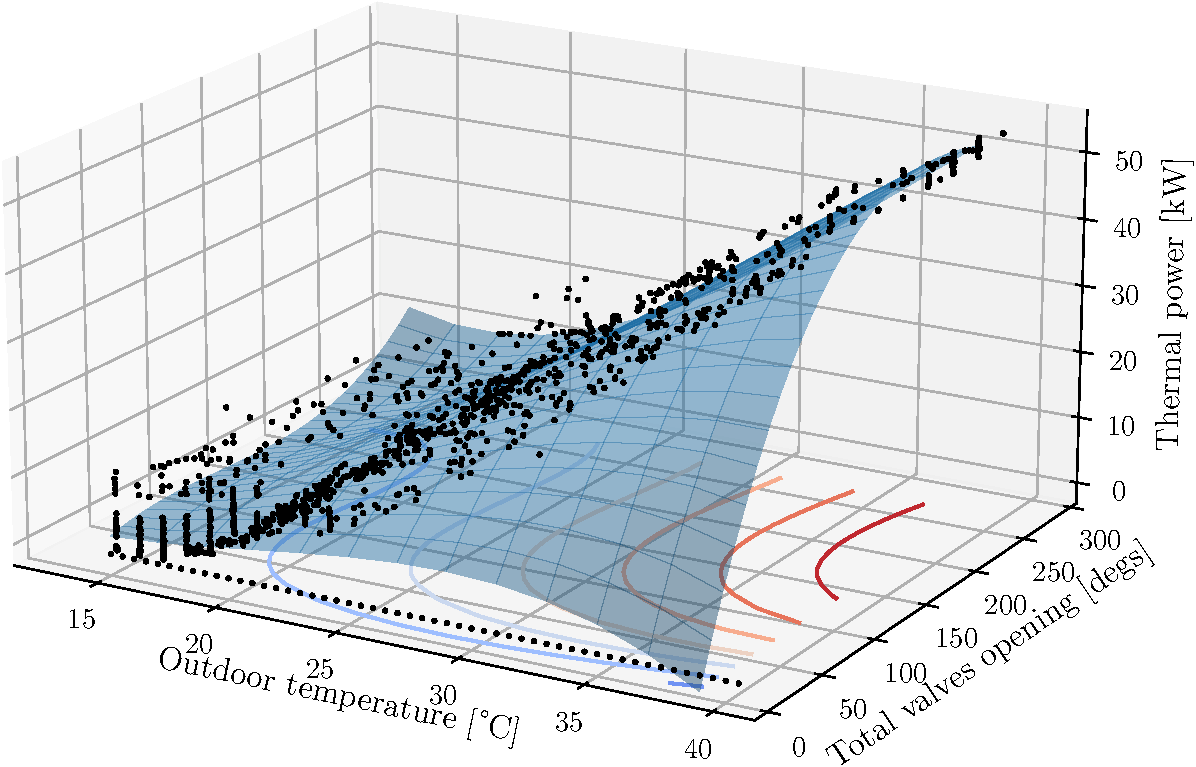
\includegraphics[width=0.5\linewidth]{../images/chap3_thermal_surface.pdf}  \\[14pt]
	\hspace{10pt}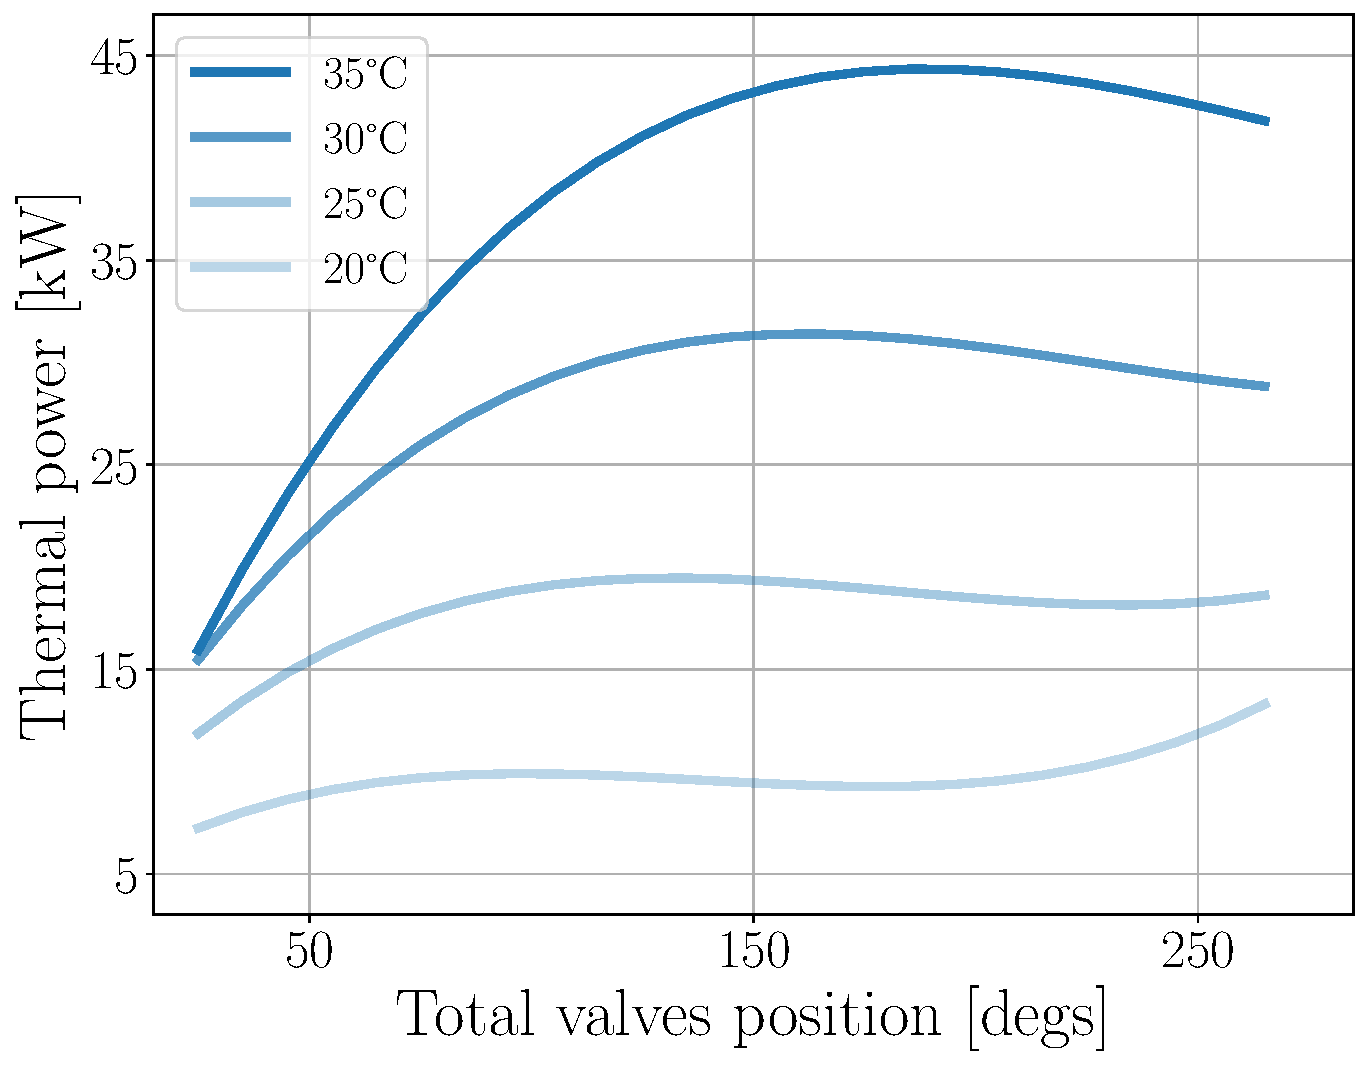
\includegraphics[width=0.4\linewidth]{../images/chap3_ther_energy.pdf} \hspace{3pt}
	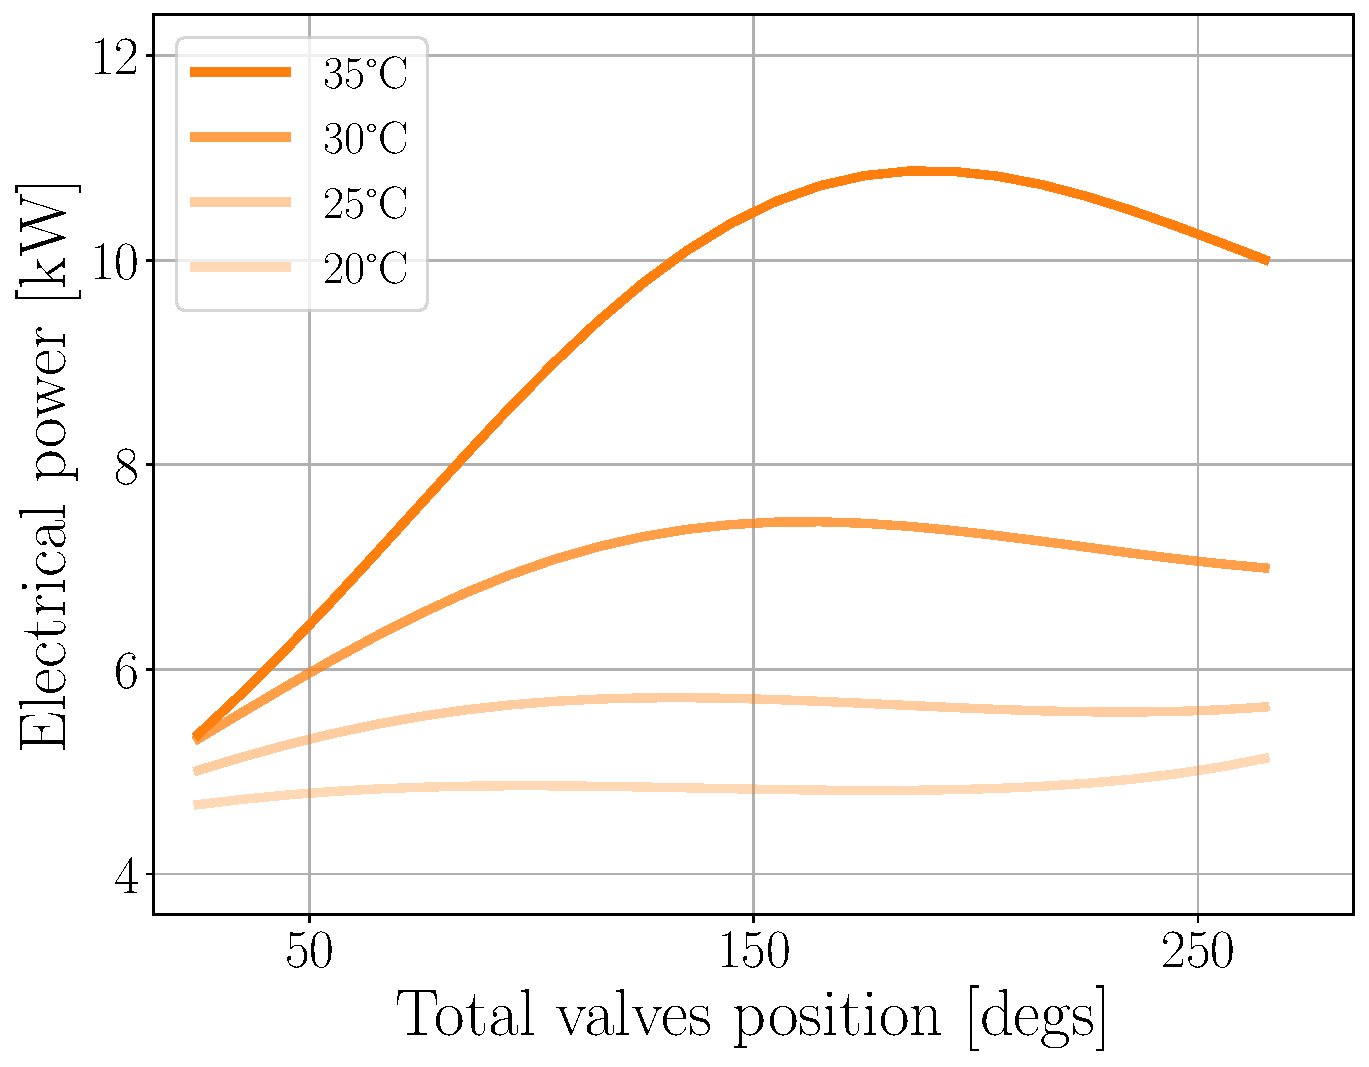
\includegraphics[width=0.4\linewidth]{../images/chap3_elec_energy.pdf}
	\caption{Reconstruction of the chiller refrigeration surface (top). Data were collected during a period of 203 hours, including both of open-loop excitation as well as closed-loop operation. Thermal power $Q(T_\text{out},\Theta)$ (bottom left) and electrical power $E(T_\text{out},\Theta)$ (bottom right) curves of the chiller as a function of the valves openings $\Theta$. The plots consider typical outdoor temperature values.}
	\label{fig.thermalAndElectrical}
\end{figure*}

Polynomial ridge regression was performed to fit the data described above. After experimenting with different model orders, we found that a cubic model provided a good balance between describing the observed points and not overfitting them. The results are presented in Figure~\ref{fig.thermalAndElectrical} and the final model was
%\begin{align}
%	&\text{Q}(T_\text{out},\Theta) = -3.15 \, T_\text{out} - 3.03 \,\texttt{e}^{-2} \, \Theta + 1.73\,\texttt{e}^{-1} \, T_\text{out}^2 \nonumber \\
%	&- 1.56\,\texttt{e}^{-3} T_\text{out} \Theta + 3.09\,\texttt{e}^{-4} \Theta^2 - 2.75\,\texttt{e}^{-3} T_\text{out}^3 \label{eq.thermalEnergy} \\
%	&+ 4.90 \,\texttt{e}^{-4} T_\text{out}^2 \Theta - 6.86 \,\texttt{e}^{-5} T_\text{out} \Theta^2 + 2.56 \,\texttt{e}^{-6}\Theta^3 + 20.22 \nonumber
%\end{align}
\begin{align}
	&\text{Q}(T_\text{out},\Theta) = 20.22 -3.15 \, T_\text{out} - 3.03 \,\texttt{e}^{-2} \, \Theta + 1.73\,\texttt{e}^{-1} \, T_\text{out}^2 - 1.56\,\texttt{e}^{-3} T_\text{out} \Theta \nonumber \\
	& + 3.09\,\texttt{e}^{-4} \Theta^2 - 2.75\,\texttt{e}^{-3} T_\text{out}^3 + 4.90 \,\texttt{e}^{-4} T_\text{out}^2 \Theta - 6.86 \,\texttt{e}^{-5} T_\text{out} \Theta^2 + 2.56 \,\texttt{e}^{-6}\Theta^3  \label{eq.thermalEnergy} 
\end{align}
with \texttt{e}$^{n}$ being a shorthand for $\times10^{n}$. The model attained a mean absolute error of $2.88$ and a mean squared error of $12.97\,$kW. As a second step, we fit a concave coefficient of performance (COP) curve, which is typical for variable-speed compressor chillers and dictates how efficient they are in converting electrical to thermal energy. The final utilized COP curve was
%It was assumed that the passive cooling load imposed by the remaining surgery center rooms was such that the vertical range in Figure~\ref{fig.thermalAndElectrical} mapped to the increasing part of the COP curve, the peak, as well as the decreasing section. We did so intentionally to pose a challenging optimization objective and assess the capabilities of the proposed control scheme. 
\begin{equation}
		%		\text{COP}(Q) = 3.30 \, \texttt{e}^{-7} Q^4 - 2.69 \, \texttt{e}^{-5} Q^3 - 2.67 \, \texttt{e}^{-3} Q^2 + 2.34 \, \texttt{e}^{-1} Q^1 - 4.45 \, \texttt{e}^{-4}
		\text{COP}(Q) =  - 4.45 \, \texttt{e}^{-4}  + 2.34 \, \texttt{e}^{-1} Q - 2.67 \, \texttt{e}^{-3} Q^2 - 2.69 \, \texttt{e}^{-5} Q^3 + 3.30 \, \texttt{e}^{-7} Q^4
		\label{eq.COP}
\end{equation}
which, given the thermal range displayed in Figure~\ref{fig.thermalAndElectrical}, implies in a performance coefficient varying approximately between 1.5 and 4.5.

With the thermal model \eqref{eq.thermalEnergy} and the COP curve \eqref{eq.COP} at hand, the electrical power could be calculated according to $E = Q(T_\text{out},\Theta)/\text{COP}(Q(T_\text{out},\Theta))$, measured in kW. Several slices of the thermal power surface, and their associated electrical power counterparts are presented in Figure~\ref{fig.thermalAndElectrical}. The plots illustrate how the curves change depending on the outdoor temperature, and how strongly the electrical power profile is affected by this external factor. In particular, one notices that when the outside temperature is high, it is more economic to open the valves and increase the chilled water flow rather than keeping them partially closed. Clearly though, the real-time optimal position for them will depend on the system dynamics, the desired temperature envelope and the external disturbances.

\section{MPC formulation and numerical computations}

Given the learned GP models $\mu_i$, $i=1,2,3$ described in \eqref{eq.GPmodels}, a given maximum temperature $T_{\max}$, and our reconstructed electrical power surface, we formulate the following optimization problem to control the valves $\theta_i$ while reducing the chiller energy consumption $E_t$
\begin{subequations}
	\begin{align}
		\min & \quad \sum_{t=0}^{N-1}  \left(E_t + \rho \Delta_t \right) + \rho_N \Delta_N\\
		\text{s.t.}
		& \quad T_{t+1} = \mu(T_t,\theta_t,T_{\text{sup}},T_{\text{out}}) \label{eq.constr1} \\
		& \quad T_t + \beta \, \text{var}^{1/2} (T_t,\theta_t,T_{\text{sup}},T_{\text{out}}) \leq T_\text{max} + \delta_t \label{eq.constr2} \\
		& \quad E_t = Q(T_\text{out},\Theta_t) / \, \text{COP}(Q(T_\text{out},\Theta_t)) \label{eq.constr3} \\
		& \quad \theta_{\text{min}} \leq \theta_t \leq \theta_{\text{max}} \label{eq.constr4} \\
		& \quad \delta_t \geq 0 \label{eq.constr5}
	\end{align}
	\label{eq.optControlProb}%
\end{subequations}
where $\Theta_t = \sum_{i=1}^{3} \theta_{i,t}$ is the sum of all valve positions. The variables $\delta_t$ in \eqref{eq.constr2} are positive slacks introduced to avoid infeasibility. If needed, these can relax the temperature constraint so that the solver can return a viable control plan. Of course, their use is heavily penalized in the objective, where $\Delta_t = \sum_{i=1}^{3} \delta_{i,t}^2$ and $\rho$, $\rho_N$ are large constants, which in our case were respectively set to $100$ and $200$. The temperature constraint \eqref{eq.constr2} also accounts for prediction uncertainty as it includes the standard deviation $\text{var}^{1/2}$. Its use confers on the formulation a risk-aware quality and robustifies the closed-loop operation. The degree of conservativeness is controlled by the constant $\beta$, chosen to be $2$ as in Figure~\ref{fig.trainTestRes}. The prediction horizon was set to $N=12$ steps, which translates to 2 hours. As suggested by our notation, $T_\text{out}$ and $T_\text{sup}$ were kept constant throughout all prediction steps--but updated from one sampling period to the next. Finally, our maximum temperature value was $T_{\max} = 21$ degrees Celsius.

The optimization problem \eqref{eq.optControlProb} was written in \texttt{Python} with the aid of CasADi \citep{casadi}, an automatic-differentiation package that provides gradient information for numerical solvers--in our case, the interior-point method IPOPT. As is customary in predictive control, \eqref{eq.optControlProb} was recursively solved on-line with the most recently available system information, with only the first optimal control action being transmitted to the valves. We underline that the main source of complexity in \eqref{eq.optControlProb} is the presence of the constraints \eqref{eq.constr1} and \eqref{eq.constr2}, which are highly non-linear due the GP mean and variance. Since convexity is absent, multiple local optima might exist, a fact that was indeed verified in practice. By intelligently providing solvers with high-quality initial guesses, this problem can be mostly overcome. Our particular case study relied on initializing the numerical solver with control, temperature, slack and energy trajectories obtained with a virtual PI controller. The intuition was to allow the MPC loop to build on such an initial guess and further optimize operation. For a detailed study on solve times and how the number of GP data-points impacted them, see Appendix~A.

In order to shed light on how the number of training points affects the solve times of the non-convex optimization problem \eqref{eq.optControlProb}, the following study was conducted. Five sets of GP models were trained on distinct datasets with cardinalities $N = 352$, $794$ (precisely the one used in the experiments), $1280$, $1910$ and $2643$. In all scenarios, the total number of points present in each of the GPs was approximately a third of the total number $N$, so that the models were balanced. We then generated random initial conditions, uniformly sampled from sensible intervals: $16 \leq T_{1,2,3} \leq 23$, $9 \leq T_\text{sup} \leq 13$, and $15 \leq T_\text{out} \leq 35$. Finally, we solved the warm-started non-convex MPC \eqref{eq.optControlProb} on a 2.4 GHz, i9 machine $50$ times per scenario and recorded their run times. 

The results are presented in Figure~\ref{fig.runTimes}, where the vertical scale is logarithmic. The median values of the box plots rose from $4.19$ to $18.69$, $85.42$, $121.12$ and $255.68$ seconds respectively from the smallest to the largest dataset. Although using $N=1910$ points does not seem unreasonable at first, challenging initial conditions such as ones close to violating constraints can easily increase the problem solve time: the highest point obtained for the $N=1910$ scenario was $429$ seconds. Ideally, and specially when occupants experience thermal discomfort, the control action has to be computed in negligible time to be applied as soon as possible to the system. Keeping the solve times below a low percentile of the total sampling period is thus a common desideratum. In our application, we regarded $N=794$ to be an adequate choice.
%Recalling that ideally the control action has to be computed in negligible time, one concludes that this scenario is infeasible for practical deployment. Indeed, if the solve time is $429$ secs and our sampling period is $600$ secs, the control action will only be applied for 28\% of the total time.

\begin{figure}[!t]
	\centering
	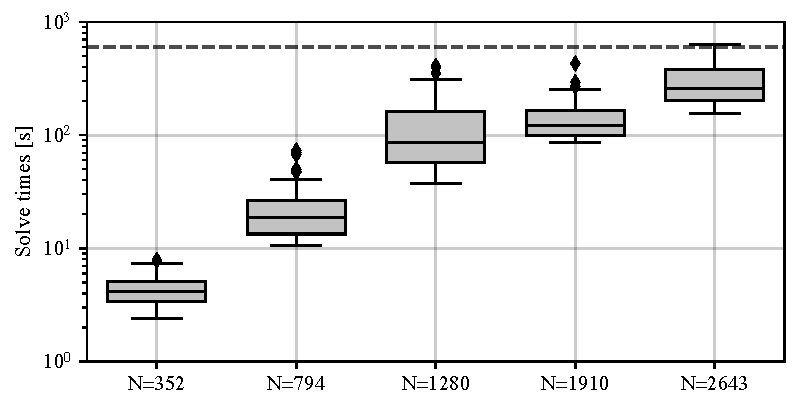
\includegraphics[scale=0.67]{../images/chap3_warm_start.pdf} \hspace{6pt}
	\caption{Box and whisker plots of the MPC solve times considering different dataset sizes. The dashed gray line marks our sampling period of $10\,$mins. Each boxplot is based on 50 time samples, obtained using randomized initial conditions.}
	\label{fig.runTimes}
\end{figure}

\section{Experimental results}

The previously described Gaussian process-based MPC formulation was deployed on the local computer and used to operate the surgery center cooling system during multiple days in the months of October and November 2021. We report in Figure~\ref{fig.prettyCool} a four-day uninterrupted experiment carried out from November 10 to November 13 that is rather representative of the local internal and external conditions. We highlight that the curves displayed in the figure were not filtered in any way; the sole manipulation performed with the data was the imputation of the missing temperature entries using linear interpolation. These points, however, accounted for only 43 out of the 1'728 indoor temperature values gathered during the four-day experiment. The first and third top plots show the room temperatures and the immediate uncertainty associated with the GP predictions $T_\text{unc} = \beta \text{var}^{1/2}$ as employed in the formulation \eqref{eq.constr2}. The second plot displays the valve positions, that is, the control variables. Both outdoor signals, the external temperature and the solar radiation are also given. The reader is reminded that, although the latter contributes with additional heat gains, it is completely unknown to the controller as explained in Section~\ref{sec.ModelTrainingAndTesting}. Lastly, the bottom plot shows the supply water temperature $T_\text{sup}$, an external disturbance that was incorporated in the GP models. This signal evolves according to the chiller own dynamics, over which we had no direct control.

\afterpage{
\begin{landscape}
\begin{figure}[!t]
	\centering
	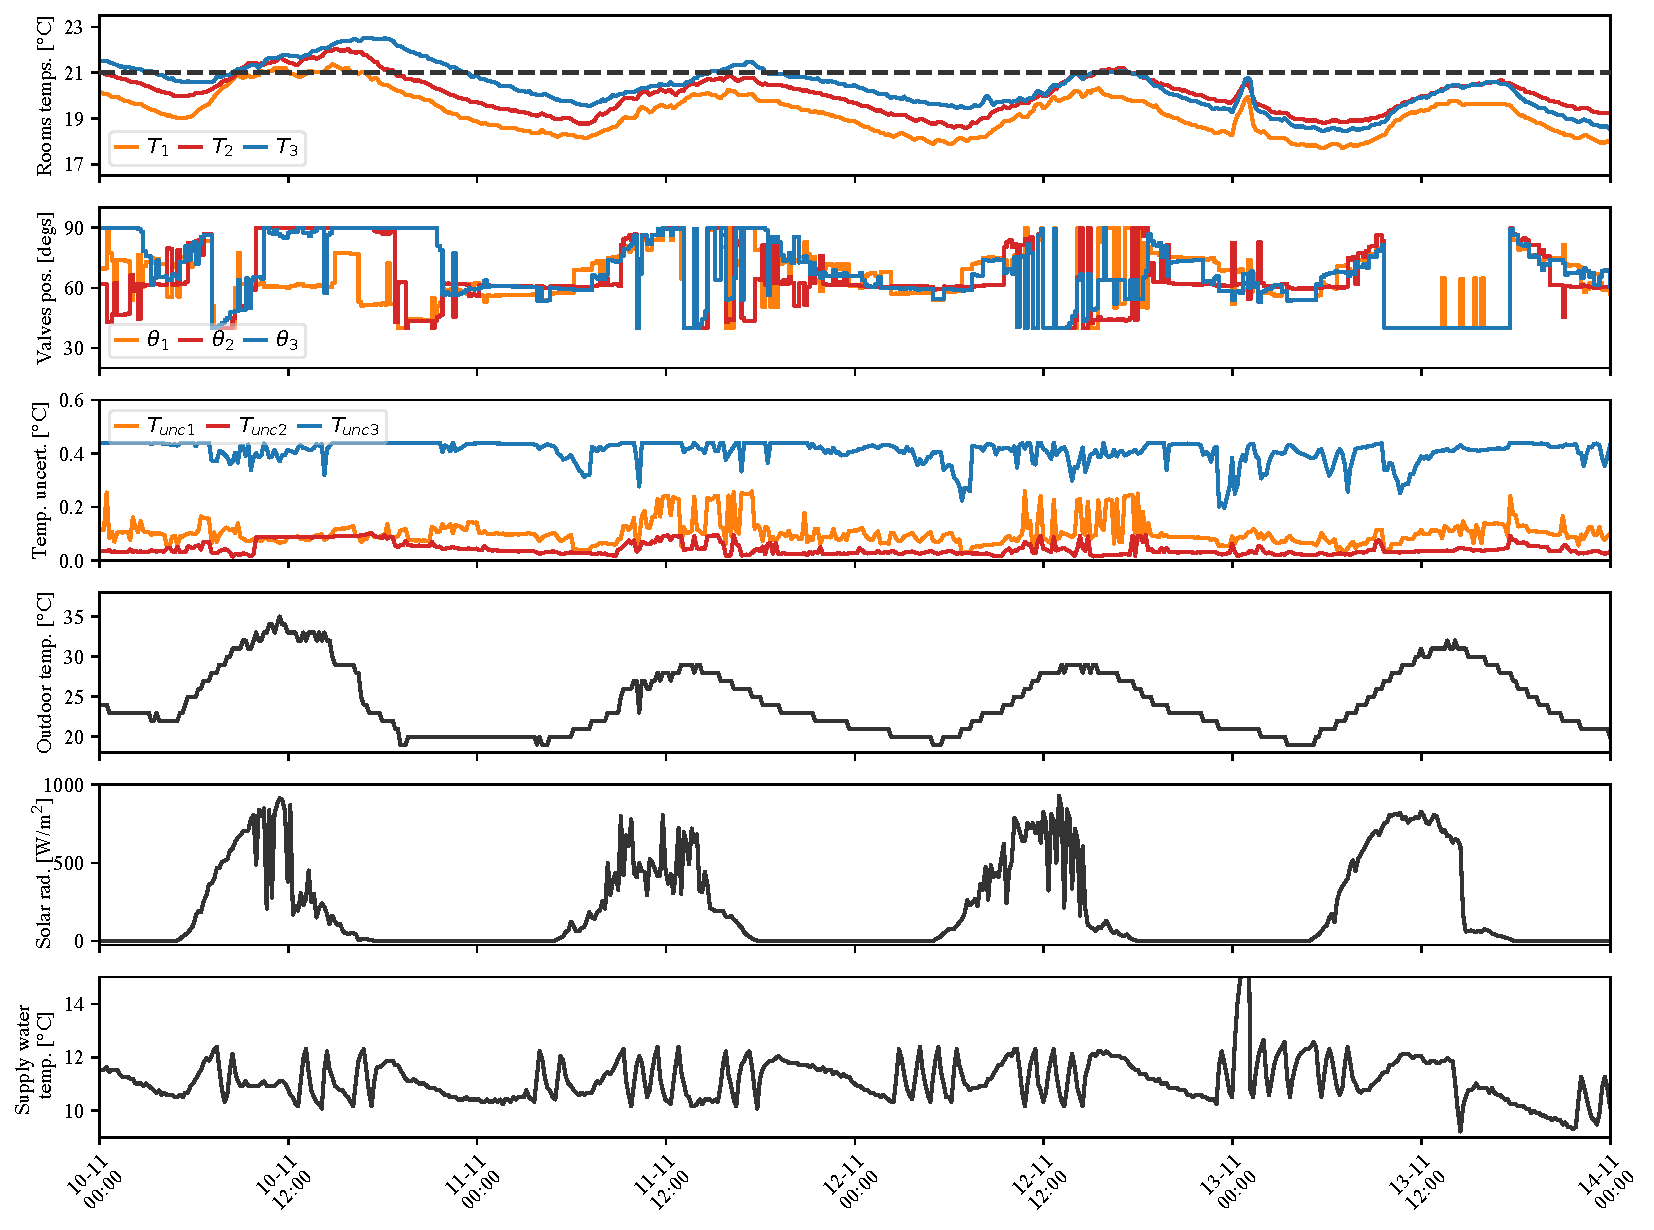
\includegraphics[width=0.7\linewidth]{../images/chap3_expres.pdf} 
	\caption{MPC experimental results over four days: indoor temperature, valve position and uncertainty estimate associated with each room (top three plots); outdoor temperature, solar radiation and \acp{ahu} supply water temperature (bottom three plots). The system was sampled and controlled with a periodicity of 10 minutes.}
	\label{fig.prettyCool}
\end{figure}	
\end{landscape}
}

Consider first the day, November 10, and note the relatively high room temperatures when the experiment started, which were the consequence of a harsh previous day. The MPC controller made use of some control authority to bring the temperatures below the 21-degree line before partially closing the valves. After the morning shift started (7 am), even though $\theta_2$ and $\theta_3$ were fully open, $T_2$ and $T_3$ violated the constraints and were only brought below 21 degrees late that evening. High initial conditions along with a peak outdoor temperature of 35 degrees overloaded the cooling system, causing violations of the indoor temperature constraint in two rooms. With regard to $T_1$, it raised quickly from 19 to 21 degrees before noon, but then stayed essentially constant at the 21-degree mark for several hours before being lowered during the evening.

The two days that followed, November 12 and 13, were less warm and, as a result, the MPC controller successfully modulated the valves to guarantee constraint satisfaction. From the plots, one can notice how $\theta_1$, $\theta_2$ and $\theta_3$ assumed  approximately constant intermediate values (around 60 degrees) during the evenings, and were more aggressively modulated on working hours. We believe this pattern to be due to the economic objective shown in Figure~\ref{fig.thermalAndElectrical}.

Lastly, we focus on the data from November 13, where it is possible to see a sudden peak in the indoor temperatures and in $T_{\text{sup}}$ around midnight. This was caused by a momentary halt in the water pumps responsible for the chilled water circuit, an event that could be regarded as a fault from a control system perspective. During this period, as there was no water circulation through the \ac{ahu} cooling coils, there was also no refrigeration and the indoor spaces received warm air since the fans were kept on. As soon as the pumps were reactivated, the chiller immediately lowered the supply water temperature and normal operation was restored. During daytime, the indoor climate was kept within the desired limits despite the valves staying saturated at their low values, even at noon. The fact that almost no additional actuation was needed is due to that day being a Saturday, when no operations are scheduled for and the three doors present in the environment are minimally opened and closed. This showcases how strong the internal heat gains and unmeasured disturbances normally are.

To assess the efficiency gains as well as the thermal performance of the deployed strategy, MPC was compared to alternative algorithms, all subject to exactly the same environmental conditions by means of simulations. We underline that this simulation model was calibrated on data that was \textit{not} included in the GPs training set, thus putting to test the MPC prediction capabilities. The disturbance signals $T_\text{out}$, $T_\text{sup}$ and $R_\text{sol}$ from November 10 were employed, and the indoor temperatures of the three rooms were uniformly initialized at values ranging from $17$ to $21$ degrees Celsius. The outdoor temperature profile was processed to yield three different weather scenarios: hot weather, which was exactly the same $T_\text{out}$ curve seen in Figure~\ref{fig.prettyCool}; warm weather, a $-2$°C shifted version of it, peaking at 33°C around noon; and mild weather, a $-5$°C shifted version of it, peaking at 30°C. Besides the MPC algorithm \eqref{eq.optControlProb}, the following were also tested:
\begin{itemize}
	\item An MPC controller, which will be referred to as REF, with perfect prediction capabilities, perfect disturbance information ($T_\text{out}$ and $T_\text{sup}$) and a long prediction horizon of five hours.
	\item PI controllers featuring anti-windup schemes and feedforward components to enhance their performance.
	\item Rule-based ON/OFF controllers that set the valves respectively to $\theta_\text{min}$ and $\theta_\text{max}$ if the indoor temperatures were below or above the set-point. 
	\item An average $(\theta_\text{max}-\theta_\text{min})/2$ controller (AVG) whose instantaneous values are selected by sampling the interval $\theta_\text{min}$ to $\theta_\text{max}$ using a uniform distribution.
\end{itemize}

\begin{figure*}[!t]
	\centering
	\hspace{0pt}
	%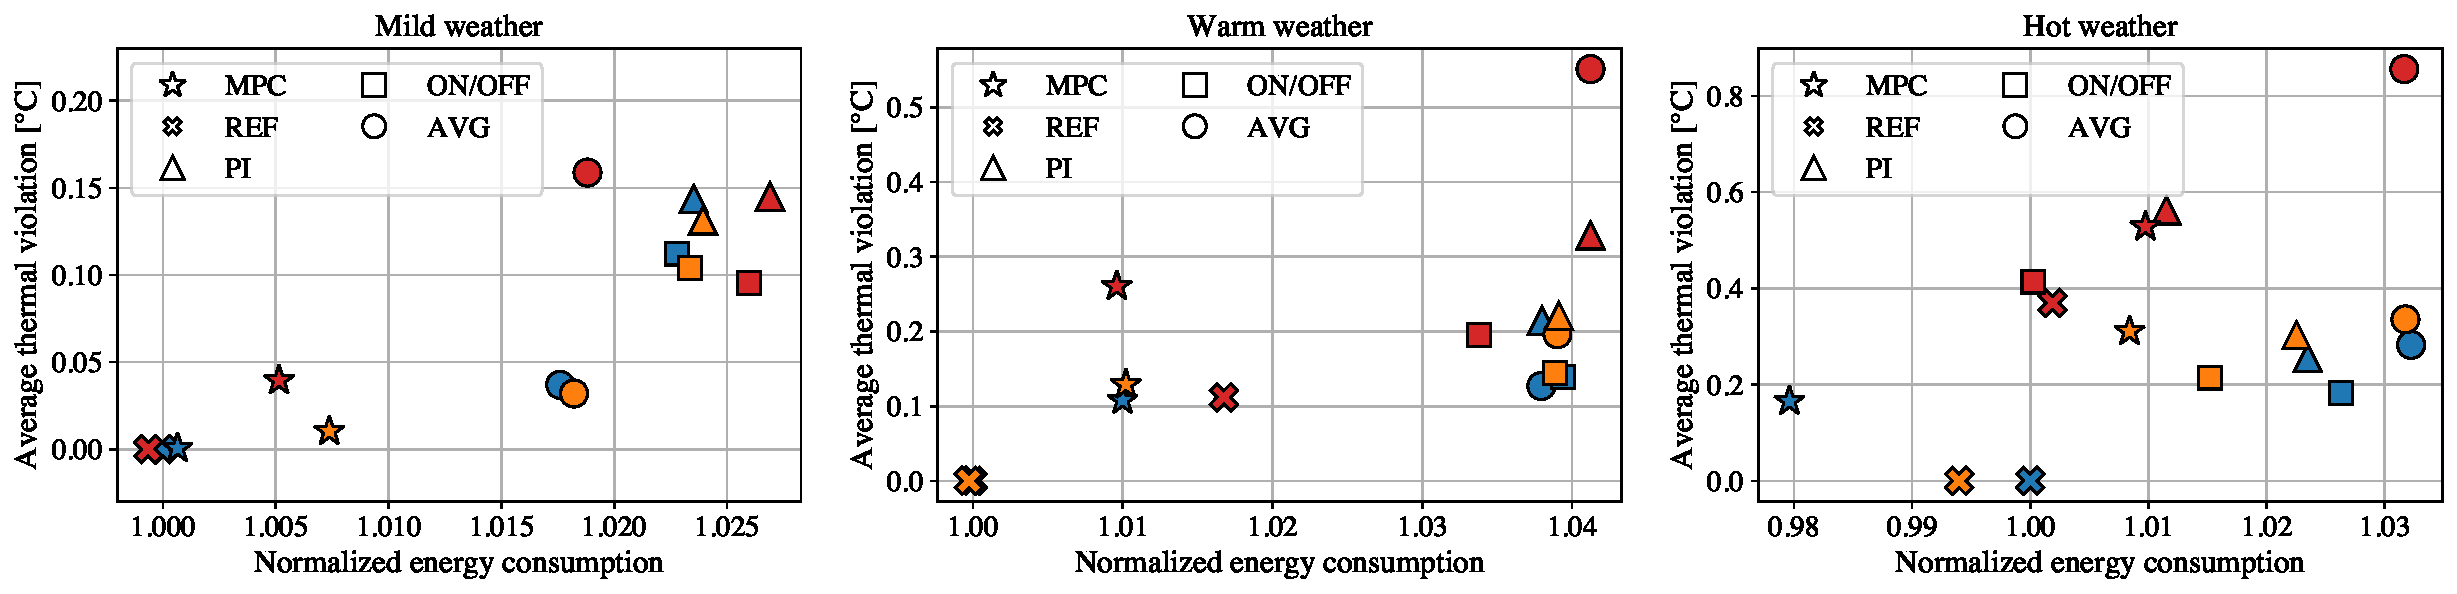
\includegraphics[width=0.95\linewidth]{../images/chap3_simres.pdf} 
	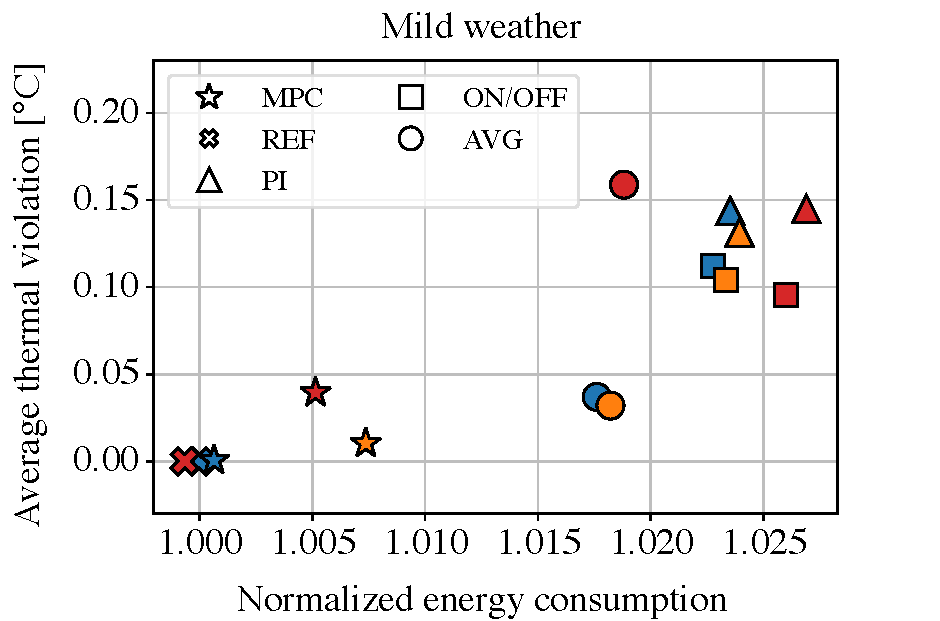
\includegraphics[width=0.55\linewidth]{../images/chap3_simres_mild.pdf} \\[12pt]
	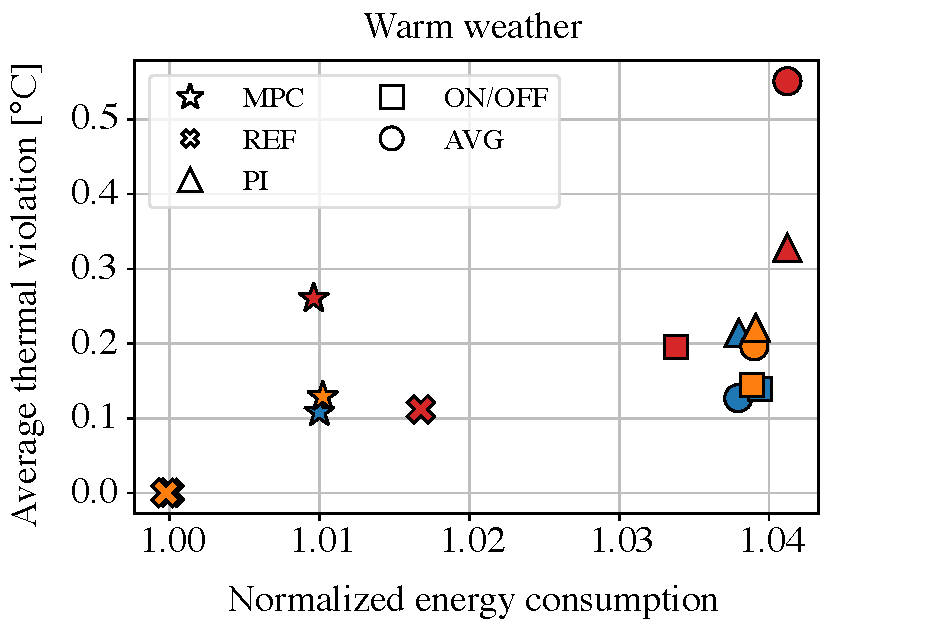
\includegraphics[width=0.55\linewidth]{../images/chap3_simres_warm.pdf} \\[12pt]
	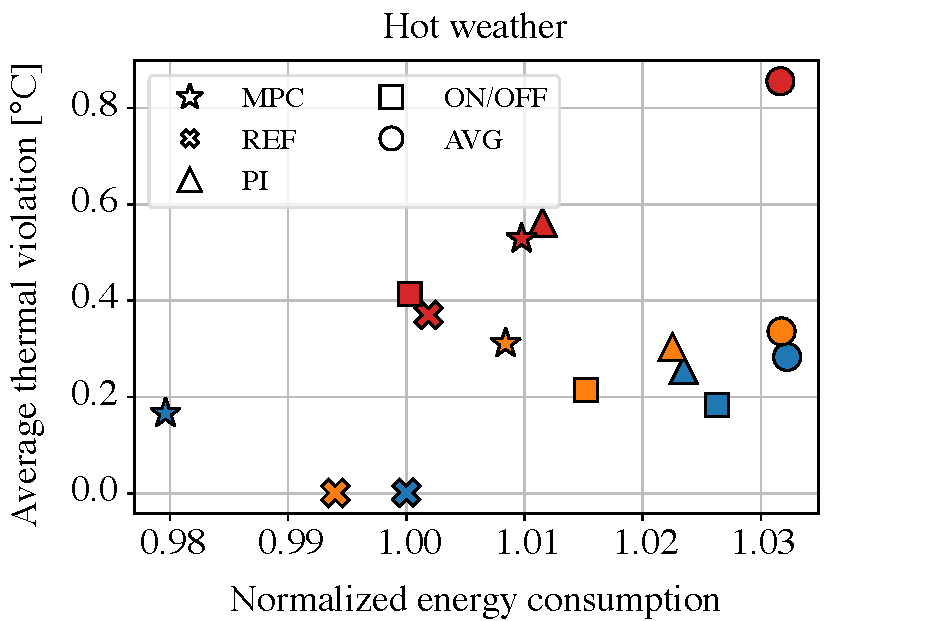
\includegraphics[width=0.55\linewidth]{../images/chap3_simres_hot.pdf} 
	\caption{Simulation results of the normalized energy consumption and thermal performance (average temperature bound violation) of different control strategies. Three weather profiles were considered: mild, warm and hot. The indoor temperatures were initialized at three different values according to the color scheme: 17°C (blue), 19°C (orange) and 21°C (red).} 
	%{\Large \textcolor{color_20}{\textbf{-}}} 17 °C, {\Large \textcolor{color_21}{\textbf{-}}} 19 °C, {\Large \textcolor{color_22}{\textbf{-}}} 21 °C.}
	\label{fig.powerRes}
\end{figure*}

The REF strategy described above was conceived and tested precisely gauge the energy saving potential of the hospital \ac{hvac} plant. This algorithm, thanks to the way it was designed with a perfect internal model and perfect forecast of the outdoor temperature and supply water temperatures, will indicate what can be achieved realistically.
%In order to gauge the energy saving potential of the \ac{hvac} plant, we executed the REF strategy described above. This algorithm can reach significant efficiency gains while guaranteeing thermal comfort since it exploits a perfect internal model as well as perfect forecasts of the outdoor and supply water temperatures.

The obtained normalized energy consumption results and average room thermal comfort violations are shown in Figure~\ref{fig.powerRes}. Since the non-linear chiller curves described in Section~\ref{sec:learningChiller} were employed to measure the energy consumption, the reader is reminded that there is a non-trivial relationship between the weather conditions and indoor temperatures, and the final consumed energy. This aspect is due to the nature of the chiller and not the use of any particular control technique. As a last note, one specific energy normalization factor was used for each weather scenario shown in Figure~\ref{fig.powerRes} to enhance clarity.

Glancing at the mild and warm weather plots, one notices how the REF and MPC data tended to be close together, and relatively far from the PI, ON/OFF and AVG clusters. Moreover, the REF and MPC points were also mostly to the left side and vertically below the other data given the same indoor temperature conditions--thus confirming their superior performance in terms of energy efficiency and indoor climate regulation. The ON/OFF and PI controllers yielded overall similar numerical results and, surprisingly, were outperformed by the AVG scheme under mild weather and starting indoor temperatures of $17\,$°C and $19\,$°C. AVG nevertheless performed poorly under warm weather and $21\,$°C, and hot weather in general. All in all, the predictive control strategies MPC and REF yielded the best results in the mild and warm weather cases, whereas the separation among them and the other techniques became less evident under hot weather, indicating a less important advantage over classical control.

By analyzing the horizontal scales and contrasting REF to PI, ON/OFF and AVG, one concludes that this particular \ac{hvac} plant could have its efficiency boosted by approximately 2.5\%, 4\% and 5\% respectively in the mild, warm and hot weather scenarios. Notice how, as opposed to studies such as \cite{bunning2020experimental}, these numbers refer to the electrical energy associated with a chiller, and not to a cumulative thermal energy. Moreover, as the hospital was not subject to time-varying electricity prices, the contrast among control strategies was not as stark as for instance the one reported in \cite{joe2022investigation}. The proposed MPC strategy \eqref{eq.optControlProb} attained results close to the aforementioned maximum percentages. Quantitatively, MPC lead to a maximum energy efficiency improvement of 2.29\%, 3.13\% and 4.76\% respectively in mild, warm and hot weather, with respect to the PI and ON/OFF counterparts.

\section{Conclusions and outlook}

The practical investigation presented in this chapter revolved around the use of Gaussian process models paired with MPC to autonomously control the industrial cooling system of a hospital building. The study was complex in comparison with many works found in the literature: it involved three thermal zones, multiple subsystems, two distinct sensor networks, four strong exogenous disturbances, and the direct control of low-level elements. From a computational viewpoint, expensive non-parametric models were used along with a non-convex MPC formulation, both in the cost and in the constraints, which brought about numerical challenges. All things considered, the chosen approach was able to guarantee the indoor comfort whenever enough actuation power was available, while also delivering superior energy performance when compared to alternative strategies.

During the course of the project, a large portion of time was dedicated to studying the building and the \acp{ahu}, deciding what signals to measure, and setting up the necessary hardware. The second most time-consuming task was certainly building a functional data ingestion pipeline for the GPs: applying the necessary filters, detecting non-reliable periods, and crafting the feature vectors by delaying the time-series and patching multiple experiments together. We therefore believe that the control community could greatly benefit from a reliable toolbox to design and test GP autoregressive models with ease, which would certainly further increase the popularity of this technique. 

With regard to possible future investigations, we consider exploring sparse Gaussian processes based on pseudo-inputs \citep{bauer2016understanding} to lower the computational burden of the MPC controller and allow for longer prediction horizons. Taking a step back, it would also be interesting to experimentally investigate with different combinations of models (not necessarily Gaussian processes) and training objectives to find a pair that is able to automatically reject spurious data periods, not only isolated points, and dispense with the need of a meticulous pre-processing stage. Indeed, being robust to an abnormal period of operation at training time could alleviate the workload of field engineers and help fulfill the promising an effortless modeling phase. In our view, parametric techniques such as neural networks are less sensitive as their internal constants are adjusted gradually by the data, whereas non-parametric techniques absorb the whole dataset and make use of it during inference. That said, perhaps additional (unobserved) covariates could be used to explain an abnormal trajectory, essentially acting as a disturbance model. Finally, from an \ac{hvac} systems perspective, more encompassing investigations could include the control of additional variables, e.g. the air flow delivered to the rooms, as well as the regulation of physical quantities other than the temperatures such as the indoor spaces humidity levels.

%Possible future investigations:  models/training procedures that are less sensible to spurious data/periods. The use of sparse GPs and alternative numerical methods (SQP) to speed-up online computations.
%A forced-air investigation where additional variables are controlled, e.g. the fans speed (variable-air volume) and the flow of chilled water, or with extra output variables, e.g. the humidity in each zone. Or having an electricity meter installed to precisely measure the demand and more exactly assess the economical advantages of the advanced control scheme, which would help motivate practitioners to make use of it.




